% Supplementary Material for the IEEE Transactions on Reliability submission.
% Standalone companion to main_tr.tex. All numbers identical to
% paper_ieee_access/main_access.tex (results_v2 pipeline).
% Compile: tectonic supplement_tr.tex
\documentclass[journal]{IEEEtran}
\usepackage{amsmath}
\usepackage{booktabs}
\usepackage{graphicx}
\usepackage{fontspec}
% Times text (IEEE look); math stays Computer Modern. Loaded by filename
% because the tectonic bundle exposes TeX Gyre Termes as OTF files.
\setmainfont{texgyretermes}[Extension=.otf, UprightFont=*-regular,
  BoldFont=*-bold, ItalicFont=*-italic, BoldItalicFont=*-bolditalic]
\usepackage[hidelinks]{hyperref}
\graphicspath{{./figs/}}
\emergencystretch=2em
\begin{document}

\title{Supplementary Material for\\ ``Multi-Horizon Failure-Risk Models for Battery Failure Prediction:\\ How Much Cross-Chemistry Transfer Is a State-of-Health Shortcut?''}

\author{Hussain~Touhid~Siddiquee,
        Syeda~Salsabil~Islam,
        Ariya~Jasimul~Islam,
        and~Chowdhury~Farzana~Hoque~Eshica}

\markboth{IEEE Transactions on Reliability --- Supplementary Material}%
{Siddiquee \MakeLowercase{\textit{et al.}}: Supplementary Material}

\maketitle

\section*{Contents}
This supplement contains the tables and figures omitted from the main manuscript for length: the diagnosis-versus-prognosis split (Table~\ref{tab:prog}), the factorial feature ablation (Table~\ref{tab:abl}), GRU and hazard-model transfer (Tables~\ref{tab:gru} and~\ref{tab:hazard}), monotonicity violations (Table~\ref{tab:mono}), the full SOH-ablation statistical evidence (Table~\ref{tab:sohtests}), the recalibration arms (Tables~\ref{tab:rec-r1} and~\ref{tab:rec-r2}), the leave-condition-out analysis (Table~\ref{tab:condshift}), and eleven supplementary figures. Section references of the form ``Section III-x'' point to the main manuscript.

\section*{S-I. Supplementary Tables}

\begin{table*}[!t]
\caption{Diagnosis Versus Prognosis at H=20 (ALL-LCO Source, Raw Scores): All-Rows Pooled AUC [Cell-Level CI Where Computed] Against Prognosis-Only AUC on Rows Scored While SOH$>$0.80, With the Share of Rows Scored Above Threshold. GRU and Distance-Rule Rows Are Point Estimates.}
\label{tab:prog}
\centering
\footnotesize
\begin{tabular}{lllccc}
\toprule
\textbf{Target} & \textbf{Model} & \textbf{Features} & \textbf{All rows} & \textbf{Prognosis-only} & \textbf{Frac.\ above}\\
\midrule
Severson & GRU & common, no SOH & 0.631  & 0.553  & 0.99 \\
Severson & GRU & common+SOH & 0.827  & 0.756  & 0.99 \\
Severson & LightGBM & no SOH & 0.718 [0.634,0.846] & 0.674 [0.597,0.851] & 0.99 \\
Severson & LightGBM & with SOH & 0.882 [0.786,0.990] & 0.814 [0.732,0.978] & 0.99 \\
Severson & SOH-dist rule & dist rule & 0.912  & 0.862  & 0.99 \\
Severson & SOH-dist rule & SOH-only & 0.912  & 0.862  & 0.99 \\
Severson & Random Forest & no SOH & 0.746 [0.673,0.845] & 0.705 [0.632,0.843] & 0.99 \\
Severson & Random Forest & with SOH & 0.889 [0.783,0.998] & 0.825 [0.737,0.996] & 0.99 \\
Severson & XGBoost & no SOH & 0.750 [0.692,0.835] & 0.721 [0.666,0.833] & 0.99 \\
Severson & XGBoost & with SOH & 0.896 [0.804,0.995] & 0.838 [0.760,0.991] & 0.99 \\
HNEI NMC & LightGBM & no SOH & 0.988 [0.974,0.996] & 0.905 [0.863,0.944] & 0.28 \\
HNEI NMC & LightGBM & with SOH & 0.999 [0.998,0.999] & 0.969 [0.946,0.987] & 0.28 \\
HNEI NMC & Random Forest & no SOH & 0.996 [0.994,0.999] & 0.945 [0.908,0.978] & 0.28 \\
HNEI NMC & Random Forest & with SOH & 0.999 [0.999,1.000] & 0.981 [0.970,0.993] & 0.28 \\
HNEI NMC & XGBoost & no SOH & 0.989 [0.977,0.997] & 0.908 [0.870,0.945] & 0.28 \\
HNEI NMC & XGBoost & with SOH & 0.993 [0.983,0.999] & 0.963 [0.935,0.987] & 0.28 \\
SNL NCA & LightGBM & no SOH & 0.850 [0.791,0.911] & 0.841 [0.798,0.889] & 0.63 \\
SNL NCA & LightGBM & with SOH & 0.985 [0.974,0.993] & 0.891 [0.845,0.946] & 0.63 \\
SNL NCA & Random Forest & no SOH & 0.911 [0.875,0.951] & 0.837 [0.779,0.907] & 0.63 \\
SNL NCA & Random Forest & with SOH & 0.983 [0.974,0.992] & 0.901 [0.858,0.957] & 0.63 \\
SNL NCA & XGBoost & no SOH & 0.878 [0.824,0.930] & 0.849 [0.803,0.895] & 0.63 \\
SNL NCA & XGBoost & with SOH & 0.972 [0.956,0.988] & 0.886 [0.837,0.943] & 0.63 \\
SNL NMC & LightGBM & no SOH & 0.693 [0.570,0.959] & 0.728 [0.577,0.956] & 0.60 \\
SNL NMC & LightGBM & with SOH & 0.847 [0.743,0.982] & 0.722 [0.604,0.956] & 0.60 \\
SNL NMC & Random Forest & no SOH & 0.742 [0.689,0.874] & 0.649 [0.604,0.793] & 0.60 \\
SNL NMC & Random Forest & with SOH & 0.858 [0.748,0.975] & 0.706 [0.613,0.929] & 0.60 \\
SNL NMC & XGBoost & no SOH & 0.709 [0.612,0.953] & 0.730 [0.599,0.946] & 0.60 \\
SNL NMC & XGBoost & with SOH & 0.772 [0.677,0.979] & 0.729 [0.608,0.960] & 0.60 \\
SNL LFP & LightGBM & no SOH & 0.359 [0.282,0.443] & 0.383 [0.311,0.467] & 0.97 \\
SNL LFP & LightGBM & with SOH & 0.999 [0.998,1.000] & 0.993 [0.988,0.998] & 0.97 \\
SNL LFP & Random Forest & no SOH & 0.666 [0.569,0.769] & 0.588 [0.565,0.616] & 0.97 \\
SNL LFP & Random Forest & with SOH & 0.999 [0.998,1.000] & 0.994 [0.990,0.999] & 0.97 \\
SNL LFP & XGBoost & no SOH & 0.496 [0.455,0.531] & 0.517 [0.481,0.575] & 0.97 \\
SNL LFP & XGBoost & with SOH & 0.998 [0.997,1.000] & 0.991 [0.985,0.997] & 0.97 \\
\bottomrule
\end{tabular}
\end{table*}

\begin{table*}[!t]
\caption{Factorial Feature Ablation at H=20 (XGBoost, Pooled AUC With Cell-Level Bootstrap 95\% CI). Feature Groups: SOH; Cycle Index; Sensors = Voltages, Current, Temperature, Duration.}
\label{tab:abl}
\centering
\footnotesize
\begin{tabular}{lcccccc}
\toprule
 & \multicolumn{3}{c}{\textbf{Oxford}} & \multicolumn{3}{c}{\textbf{Severson}}\\
\cmidrule(lr){2-4}\cmidrule(l){5-7}
\textbf{Feature set} & \textbf{NASA src} & \textbf{CALCE src} & \textbf{ALL src} & \textbf{NASA src} & \textbf{CALCE src} & \textbf{ALL src}\\
\midrule
full & 0.957 [0.931,0.987] & 0.850 [0.764,0.910] & 0.917 [0.878,0.965] & 0.871 [0.767,0.997] & 0.850 [0.749,0.967] & 0.896 [0.812,0.995] \\
no SOH & 0.518 [0.513,0.522] & 0.416 [0.264,0.554] & 0.429 [0.279,0.597] & 0.595 [0.510,0.726] & 0.682 [0.670,0.695] & 0.750 [0.692,0.835] \\
$-$cycle & 0.965 [0.942,0.989] & 0.967 [0.929,0.981] & 0.993 [0.954,1.000] & 0.854 [0.733,0.998] & 0.766 [0.584,0.974] & 0.774 [0.578,0.998] \\
$-$SOH$-$cycle & 0.658 [0.522,0.797] & 0.433 [0.282,0.594] & 0.388 [0.224,0.506] & 0.531 [0.433,0.680] & 0.500 [0.500,0.500] & 0.535 [0.455,0.653] \\
SOH only & 0.965 [0.942,0.989] & 1.000 [1.000,1.000] & 1.000 [1.000,1.000] & 0.834 [0.695,0.991] & 0.798 [0.638,0.978] & 0.833 [0.689,0.993] \\
cycle only & 0.541 [0.537,0.545] & 0.541 [0.537,0.545] & 0.541 [0.537,0.545] & 0.709 [0.695,0.724] & 0.694 [0.681,0.708] & 0.719 [0.704,0.735] \\
sensors & 0.658 [0.522,0.797] & 0.433 [0.282,0.594] & 0.388 [0.224,0.506] & 0.531 [0.433,0.680] & 0.500 [0.500,0.500] & 0.535 [0.455,0.653] \\
\bottomrule
\end{tabular}
\end{table*}

\begin{table}[!t]
\caption{GRU Transfer at H=20 on the Common Feature Set: Seed-Averaged Per-Cell AUC ($\pm$ SD Over Seeds 42, 1, 7).}
\label{tab:gru}
\centering
\footnotesize
\begin{tabular}{llcc}
\toprule
\textbf{Training} & \textbf{Feature set} & \textbf{Oxford} & \textbf{Severson}\\
\midrule
NASA & common w/ SOH & 0.196$\pm$0.155 & 0.998$\pm$0.003 \\
NASA & common no SOH & 0.147$\pm$0.210 & 0.987$\pm$0.015 \\
CALCE & common w/ SOH & 0.182$\pm$0.311 & 0.964$\pm$0.033 \\
CALCE & common no SOH & 0.099$\pm$0.171 & 0.479$\pm$0.451 \\
ALL LCO & common w/ SOH & 0.088$\pm$0.084 & 0.991$\pm$0.015 \\
ALL LCO & common no SOH & 0.000$\pm$0.000 & 0.893$\pm$0.131 \\
\bottomrule
\end{tabular}
\end{table}

\begin{table}[!t]
\caption{Discrete-Time Hazard Model at H=20: Transfer Performance (Pooled AUC [CI]). The Fixed-Horizon XGBoost Comparator With SOH Is in Table V of the Main Manuscript.}
\label{tab:hazard}
\centering
\scriptsize
\begin{tabular}{llcc}
\toprule
\textbf{Training} & \textbf{Model} & \textbf{Oxford} & \textbf{Severson}\\
\midrule
NASA & Hazard XGBoost & 0.971 [0.953,0.991] & 0.884 [0.786,0.998] \\
NASA & Hazard Logistic & 0.500 [0.500,0.500] & 0.607 [0.402,0.890] \\
CALCE & Hazard XGBoost & 0.466 [0.301,0.578] & 0.737 [0.711,0.774] \\
CALCE & Hazard Logistic & 0.500 [0.500,0.500] & 0.500 [0.500,0.500] \\
ALL LCO & Hazard XGBoost & 0.314 [0.135,0.457] & 0.866 [0.770,0.978] \\
ALL LCO & Hazard Logistic & 0.500 [0.500,0.500] & 0.916 [0.873,0.969] \\
\bottomrule
\end{tabular}
\end{table}

\begin{table}[!t]
\caption{Monotonicity Violations: Share of Scored Rows Where the Cumulative-Risk Ordering Fails on Raw Scores (Platt in Parentheses). The Survival Product Is Monotone by Construction (Rate 0).}
\label{tab:mono}
\centering
\scriptsize
\begin{tabular}{lllcc}
\toprule
\textbf{Setting} & \textbf{Target} & \textbf{Model} & \textbf{Raw} & \textbf{Platt}\\
\midrule
within & calce & XGBoost & 0.452 & 0.056 \\
within & nasa & XGBoost & 0.323 & 0.260 \\
transfer (calce src) & oxford & LightGBM & 0.641 & 0.004 \\
transfer (calce src) & oxford & Random Forest & 0.501 & 0.540 \\
transfer (calce src) & oxford & XGBoost & 0.565 & 0.003 \\
transfer (nasa+calce src) & oxford & LightGBM & 0.210 & 0.648 \\
transfer (nasa+calce src) & oxford & Random Forest & 0.335 & 0.305 \\
transfer (nasa+calce src) & oxford & XGBoost & 0.609 & 0.341 \\
transfer (nasa src) & oxford & LightGBM & 0.521 & 0.468 \\
transfer (nasa src) & oxford & Random Forest & 0.559 & 0.376 \\
transfer (nasa src) & oxford & XGBoost & 0.248 & 0.124 \\
transfer (calce src) & severson & LightGBM & 0.405 & 0.013 \\
transfer (calce src) & severson & XGBoost & 0.420 & 0.072 \\
transfer (nasa src) & severson & LightGBM & 0.582 & 0.537 \\
transfer (nasa src) & severson & Random Forest & 0.778 & 0.557 \\
transfer (nasa src) & severson & XGBoost & 0.958 & 0.923 \\
--- & --- & Survival product & 0.000 & 0.000 \\
\bottomrule
\end{tabular}
\end{table}

\begin{table*}[!t]
\caption{SOH Ablation Evidence (ALL-LCO Source): Pooled AUC With and Without SOH, Paired Cell-Level Bootstrap 95\% CI on the Difference (Primary), and Cycle-Level DeLong $p$-Value (Secondary; Inflated by Within-Cell Correlation).}
\label{tab:sohtests}
\centering
\footnotesize
\begin{tabular}{llccccc}
\toprule
\textbf{Target} & \textbf{Model} & \textbf{H} & \textbf{AUC w/ SOH} & \textbf{AUC w/o} & \textbf{Delta AUC [boot 95\% CI]} & \textbf{DeLong p}\\
\midrule
Oxford & XGBoost & 10 & 0.980 & 0.433 & +0.547 (CI undefined: 5 cells) & $<10^{-16}$ (underflow) \\
Oxford & XGBoost & 20 & 0.917 & 0.429 & +0.488 (CI undefined: 5 cells) & $<10^{-16}$ (underflow) \\
Oxford & XGBoost & 30 & 0.991 & 0.377 & +0.614 (CI undefined: 5 cells) & $<10^{-16}$ (underflow) \\
Oxford & XGBoost & 50 & 0.932 & 0.580 & +0.351 (CI undefined: 5 cells) & $<10^{-16}$ (underflow) \\
Oxford & LightGBM & 10 & 0.996 & 0.547 & +0.449 (CI undefined: 5 cells) & $<10^{-16}$ (underflow) \\
Oxford & LightGBM & 20 & 0.971 & 0.332 & +0.639 (CI undefined: 5 cells) & $<10^{-16}$ (underflow) \\
Oxford & LightGBM & 30 & 0.743 & 0.484 & +0.259 (CI undefined: 5 cells) & $9.7e-13$ \\
Oxford & LightGBM & 50 & 0.832 & 0.448 & +0.384 (CI undefined: 5 cells) & $<10^{-16}$ (underflow) \\
Oxford & Random Forest & 10 & 0.978 & 0.626 & +0.352 (CI undefined: 5 cells) & $<10^{-16}$ (underflow) \\
Oxford & Random Forest & 20 & 0.989 & 0.581 & +0.409 (CI undefined: 5 cells) & $<10^{-16}$ (underflow) \\
Oxford & Random Forest & 30 & 0.971 & 0.462 & +0.508 (CI undefined: 5 cells) & $<10^{-16}$ (underflow) \\
Oxford & Random Forest & 50 & 0.933 & 0.460 & +0.473 (CI undefined: 5 cells) & $<10^{-16}$ (underflow) \\
Severson & XGBoost & 10 & 0.878 & 0.741 & +0.137 [0.079, 0.249] & $<10^{-16}$ (underflow) \\
Severson & XGBoost & 20 & 0.896 & 0.750 & +0.146 [0.097, 0.233] & $<10^{-16}$ (underflow) \\
Severson & XGBoost & 30 & 0.906 & 0.745 & +0.162 [0.115, 0.237] & $<10^{-16}$ (underflow) \\
Severson & XGBoost & 50 & 0.917 & 0.736 & +0.180 [0.134, 0.250] & $<10^{-16}$ (underflow) \\
Severson & LightGBM & 10 & 0.870 & 0.736 & +0.134 [0.105, 0.200] & $<10^{-16}$ (underflow) \\
Severson & LightGBM & 20 & 0.882 & 0.718 & +0.164 [0.127, 0.227] & $<10^{-16}$ (underflow) \\
Severson & LightGBM & 30 & 0.872 & 0.771 & +0.102 [0.030, 0.230] & $<10^{-16}$ (underflow) \\
Severson & LightGBM & 50 & 0.899 & 0.744 & +0.155 [0.112, 0.214] & $<10^{-16}$ (underflow) \\
Severson & Random Forest & 10 & 0.903 & 0.740 & +0.163 [0.133, 0.225] & $<10^{-16}$ (underflow) \\
Severson & Random Forest & 20 & 0.889 & 0.746 & +0.143 [0.106, 0.226] & $<10^{-16}$ (underflow) \\
Severson & Random Forest & 30 & 0.919 & 0.748 & +0.171 [0.138, 0.232] & $<10^{-16}$ (underflow) \\
Severson & Random Forest & 50 & 0.921 & 0.746 & +0.175 [0.114, 0.264] & $<10^{-16}$ (underflow) \\
\bottomrule
\end{tabular}
\end{table*}

\begin{table*}[!t]
\caption{Arm A Recalibration on Severson Without SOH ($H{=}20$): Values Average the Three LCO Sources and Available Tree Models; ECE Uses 10 Equal-Width Probability Bins. From the Released Recalibration Study Artifacts.}
\label{tab:rec-r1}
\centering
\footnotesize
\begin{tabular}{rccccccc}
\toprule
$k$ & Zero ECE & Iso.\ ECE & Platt ECE & Temp.\ ECE & Iso.\ AUC & Platt AUC & Temp.\ AUC\\
\midrule
5 & 0.817 & 0.044 & 0.045 & 0.563 & 0.616 & 0.599 & 0.669 \\
10 & 0.817 & 0.010 & 0.010 & 0.561 & 0.634 & 0.646 & 0.651 \\
20 & 0.817 & 0.013 & 0.013 & 0.560 & 0.634 & 0.655 & 0.648 \\
40 & 0.817 & 0.015 & 0.015 & 0.561 & 0.637 & 0.657 & 0.653 \\
\bottomrule
\end{tabular}
\end{table*}

\begin{table*}[!t]
\caption{Arm B Recovery at $k=5$ on Severson Without SOH, H=20. Recovery Ratio Uses the Within-LCO Ceiling; Retention Is the LCO-Holdout AUC Before and After the Update. \textsuperscript{*}Ratio above 1.0 is a ceiling-mismatch artifact, not super-ceiling recovery (see main manuscript, Section III-H).}
\label{tab:rec-r2}
\centering
\footnotesize
\begin{tabular}{llccccc}
\toprule
\textbf{Training} & \textbf{Model} & \textbf{Zero AUC} & \textbf{Arm B AUC} & \textbf{Recovery} & \textbf{DeLong p} & \textbf{LCO retention}\\
\midrule
NASA & XGBoost & 0.620 & 0.854 & +1.04\textsuperscript{*} & $<10^{-3}$ & 1.000 $\rightarrow$ 1.000 \\
NASA & LightGBM & 0.493 & 0.838 & +0.88 & $<10^{-3}$ & 1.000 $\rightarrow$ 0.997 \\
NASA & Random Forest & 0.724 & 0.751 & +0.19 & $<10^{-3}$ & 0.959 $\rightarrow$ 0.314 \\
CALCE & XGBoost & 0.686 & 0.796 & +0.53 & $<10^{-3}$ & 0.997 $\rightarrow$ 0.996 \\
ALL LCO & XGBoost & 0.760 & 0.828 & +0.47 & $<10^{-3}$ & 0.690 $\rightarrow$ 0.567 \\
\bottomrule
\end{tabular}
\end{table*}

\begin{table}[!t]
\caption{Leave-Condition-Out Versus Mixed-Cell Folds at H=20 (XGBoost). Conditions Are Temperature Band, C-Rate, or Both; Metadata Never Enters the Features. Ref.\ Is the Ordinary Mixed-Cell AUC for the Same Feature Set (--- Where Unstable or Not Run).}
\label{tab:condshift}
\centering
\scriptsize
\begin{tabular}{llcccc}
\toprule
\textbf{Group} & \textbf{Held-out axis} & \textbf{With SOH} & \textbf{Ref.} & \textbf{No SOH} & \textbf{Ref.}\\
\midrule
SNL NCA & temp $\times$ rate & 0.989  & 0.985 & 0.894  & 0.928 \\
SNL NCA & temperature & 0.989  & 0.985 & 0.888  & 0.928 \\
SNL NCA & C-rate & 0.961  & 0.985 & 0.820  & 0.928 \\
SNL NMC & temp $\times$ rate & 0.847  & --- & 0.666  & --- \\
SNL NMC & temperature & 0.787  & --- & 0.569  & --- \\
SNL NMC & C-rate & 0.847  & --- & 0.666  & --- \\
SNL LFP & temp $\times$ rate & 0.991  & 0.994 & --- & --- \\
SNL LFP & temperature & 0.995  & 0.994 & --- & --- \\
SNL LFP & C-rate & 0.994  & 0.994 & --- & --- \\
\bottomrule
\end{tabular}
\end{table}

\section*{S-II. Supplementary Figures}

\begin{figure}[!t]
\centering
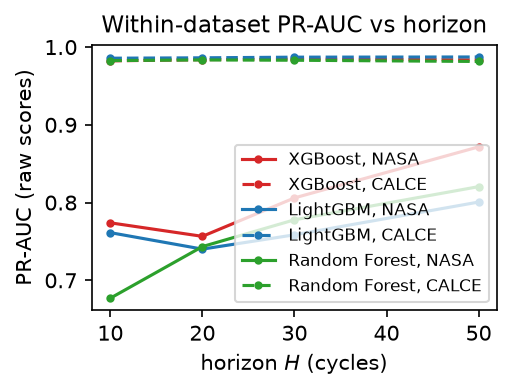
\includegraphics[width=\columnwidth]{fig_prauc_horizon.png}
\caption{Within-dataset PR-AUC of raw scores versus horizon (main manuscript, Section III-B). Precision--recall performance, unlike ROC-AUC, is sensitive to the horizon-dependent failure prevalence; it is also where isotonic's tied step outputs pay for their ranking-free compression.}
\label{fig:prauc}
\end{figure}

\begin{figure}[!t]
\centering
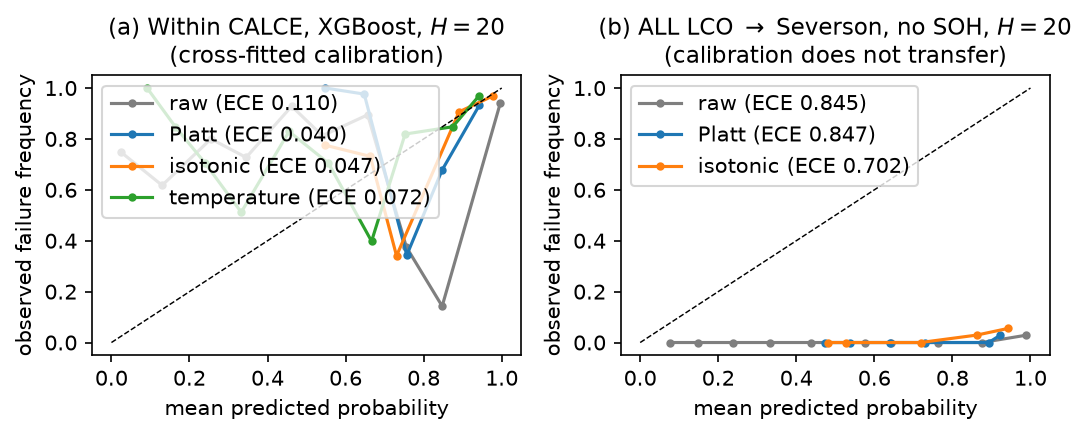
\includegraphics[width=\columnwidth]{fig_reliability_v2.png}
\caption{Reliability diagrams under the cross-fitted protocol. (a) Within CALCE, XGBoost at $H{=}20$: the fitted Platt sigmoid preserves ranking but washes confidence toward the base rate. (b) ALL-LCO $\to$ Severson without SOH at $H{=}20$: no fitted calibrator, whichever source scores it is applied to, repairs calibration on the shifted target.}
\label{fig:cal}
\end{figure}

\begin{figure}[!t]
\centering
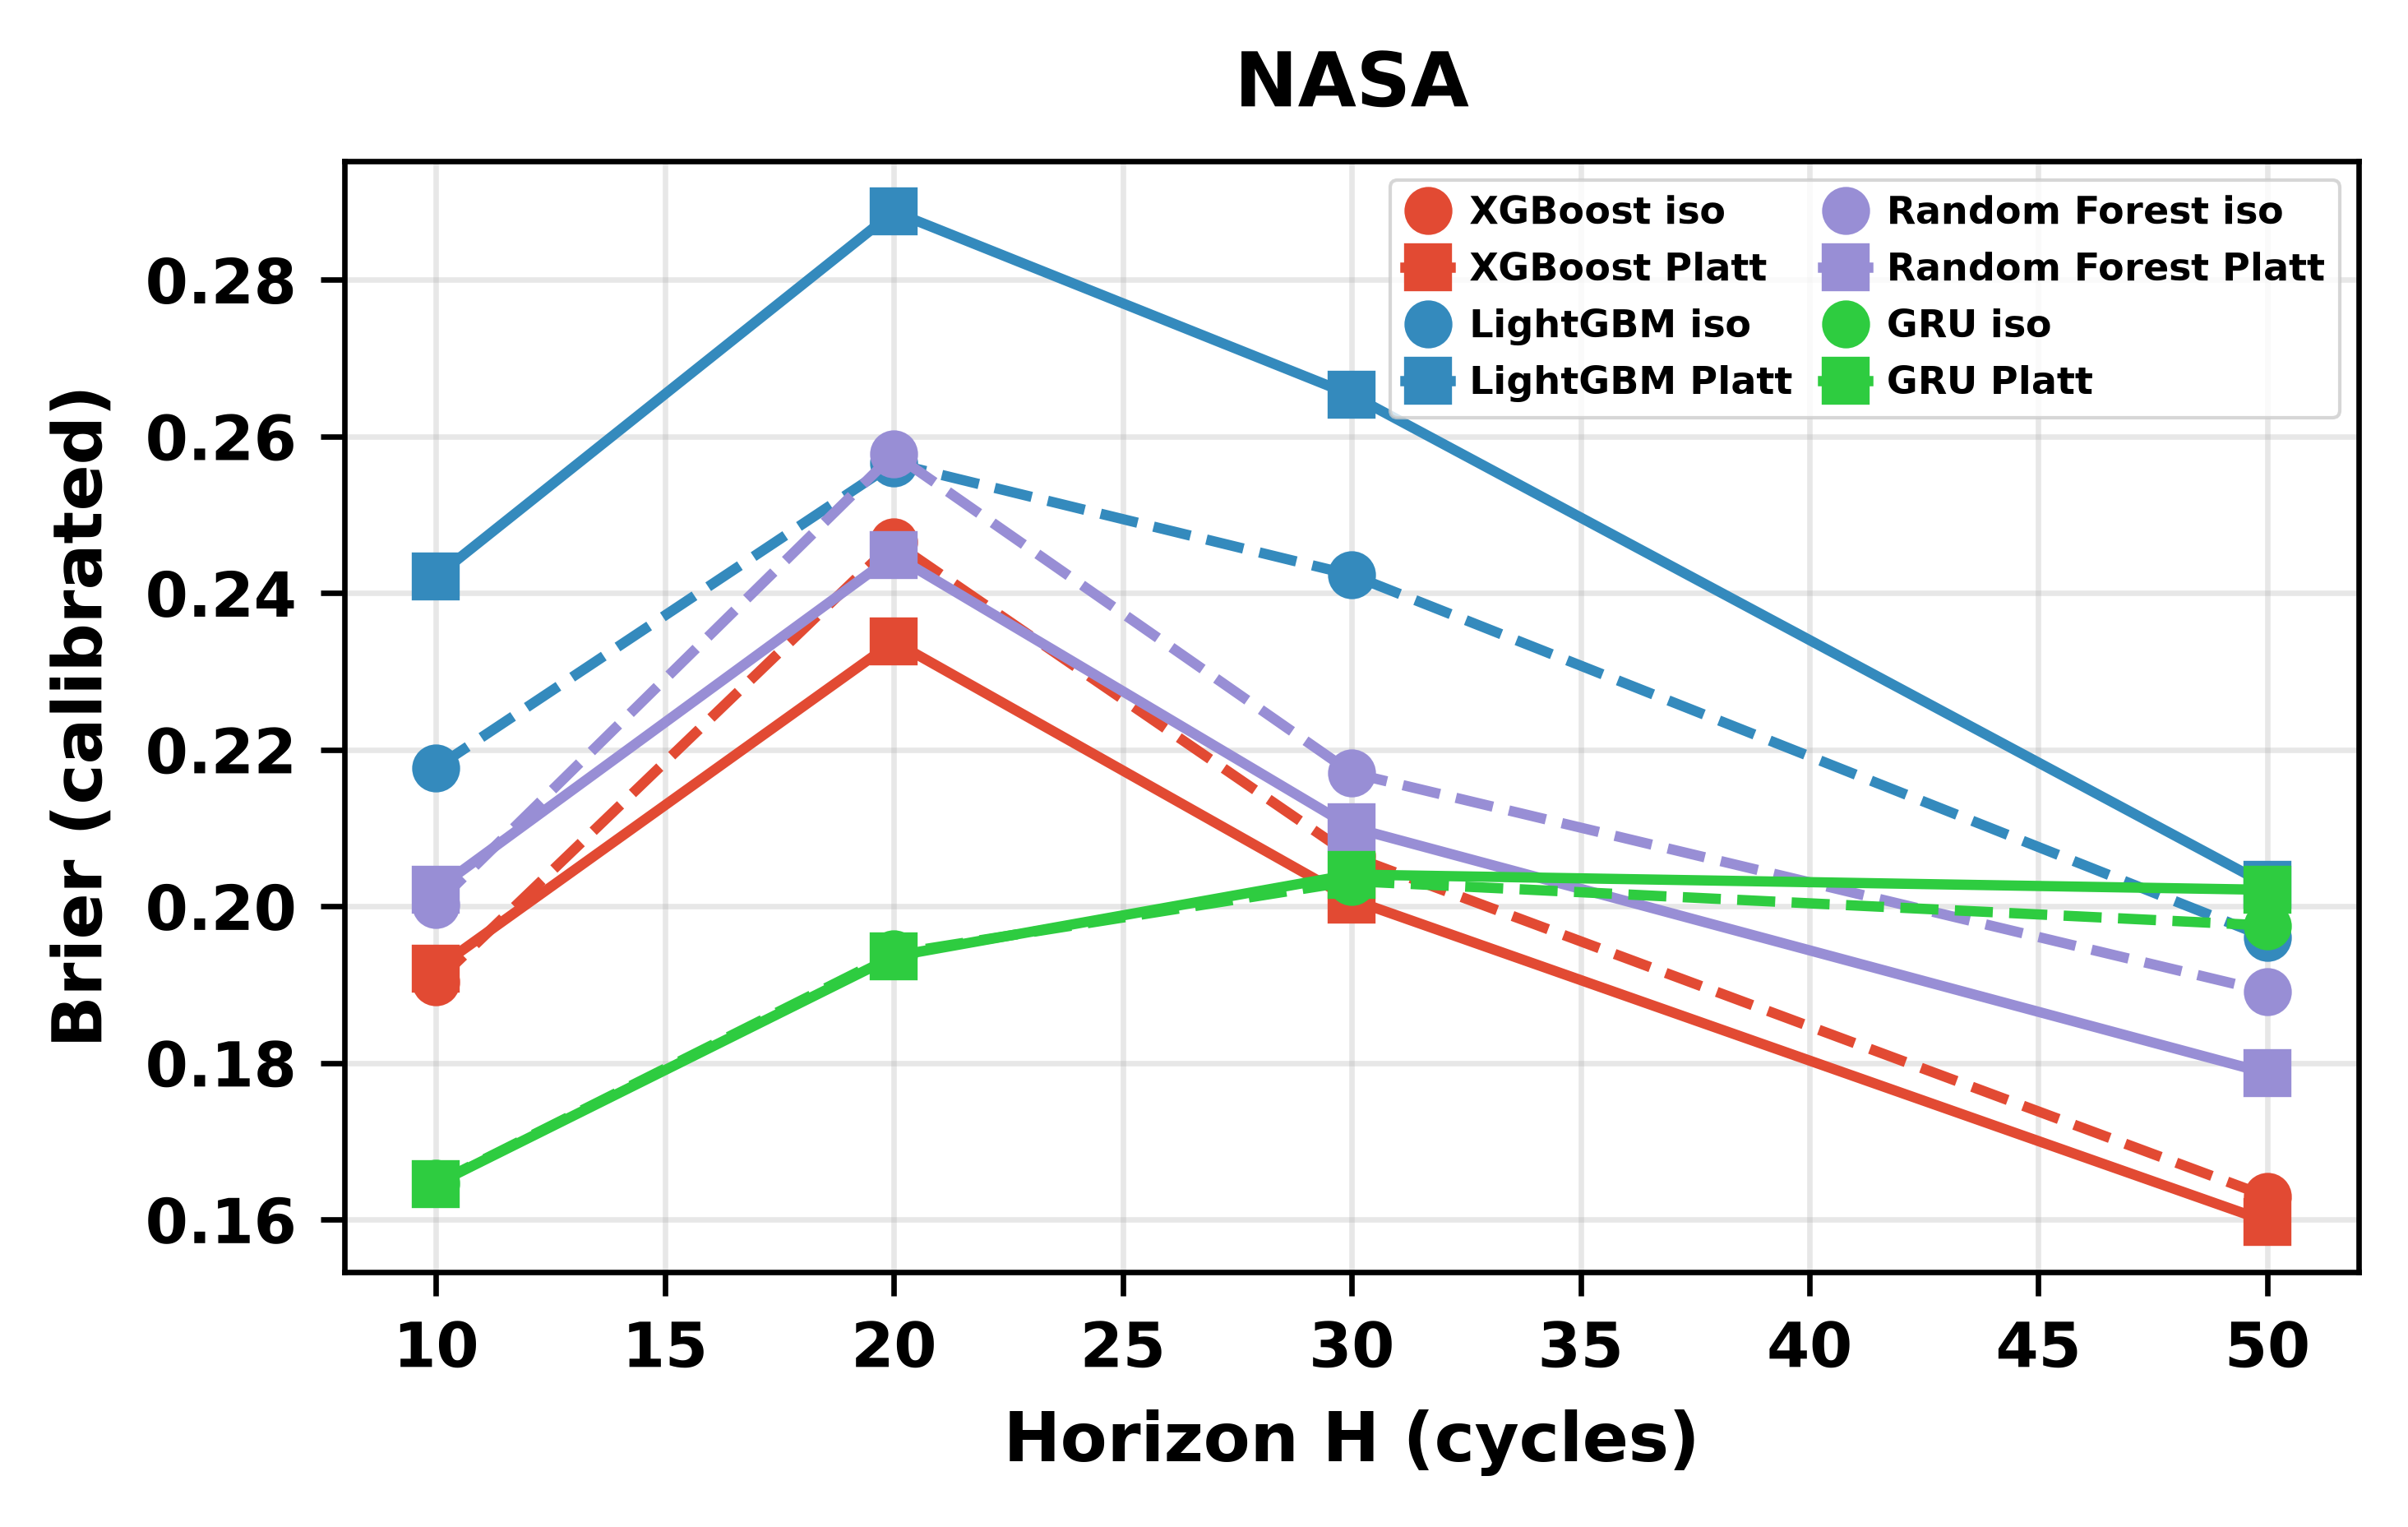
\includegraphics[width=\columnwidth]{Fig02a_Calibration_NASA.png}
\caption{Calibration curves on NASA at $H{=}20$: raw, Platt, isotonic, and temperature-scaled scores against the observed failure frequency.}
\label{fig:calnasa}
\end{figure}

\begin{figure}[!t]
\centering
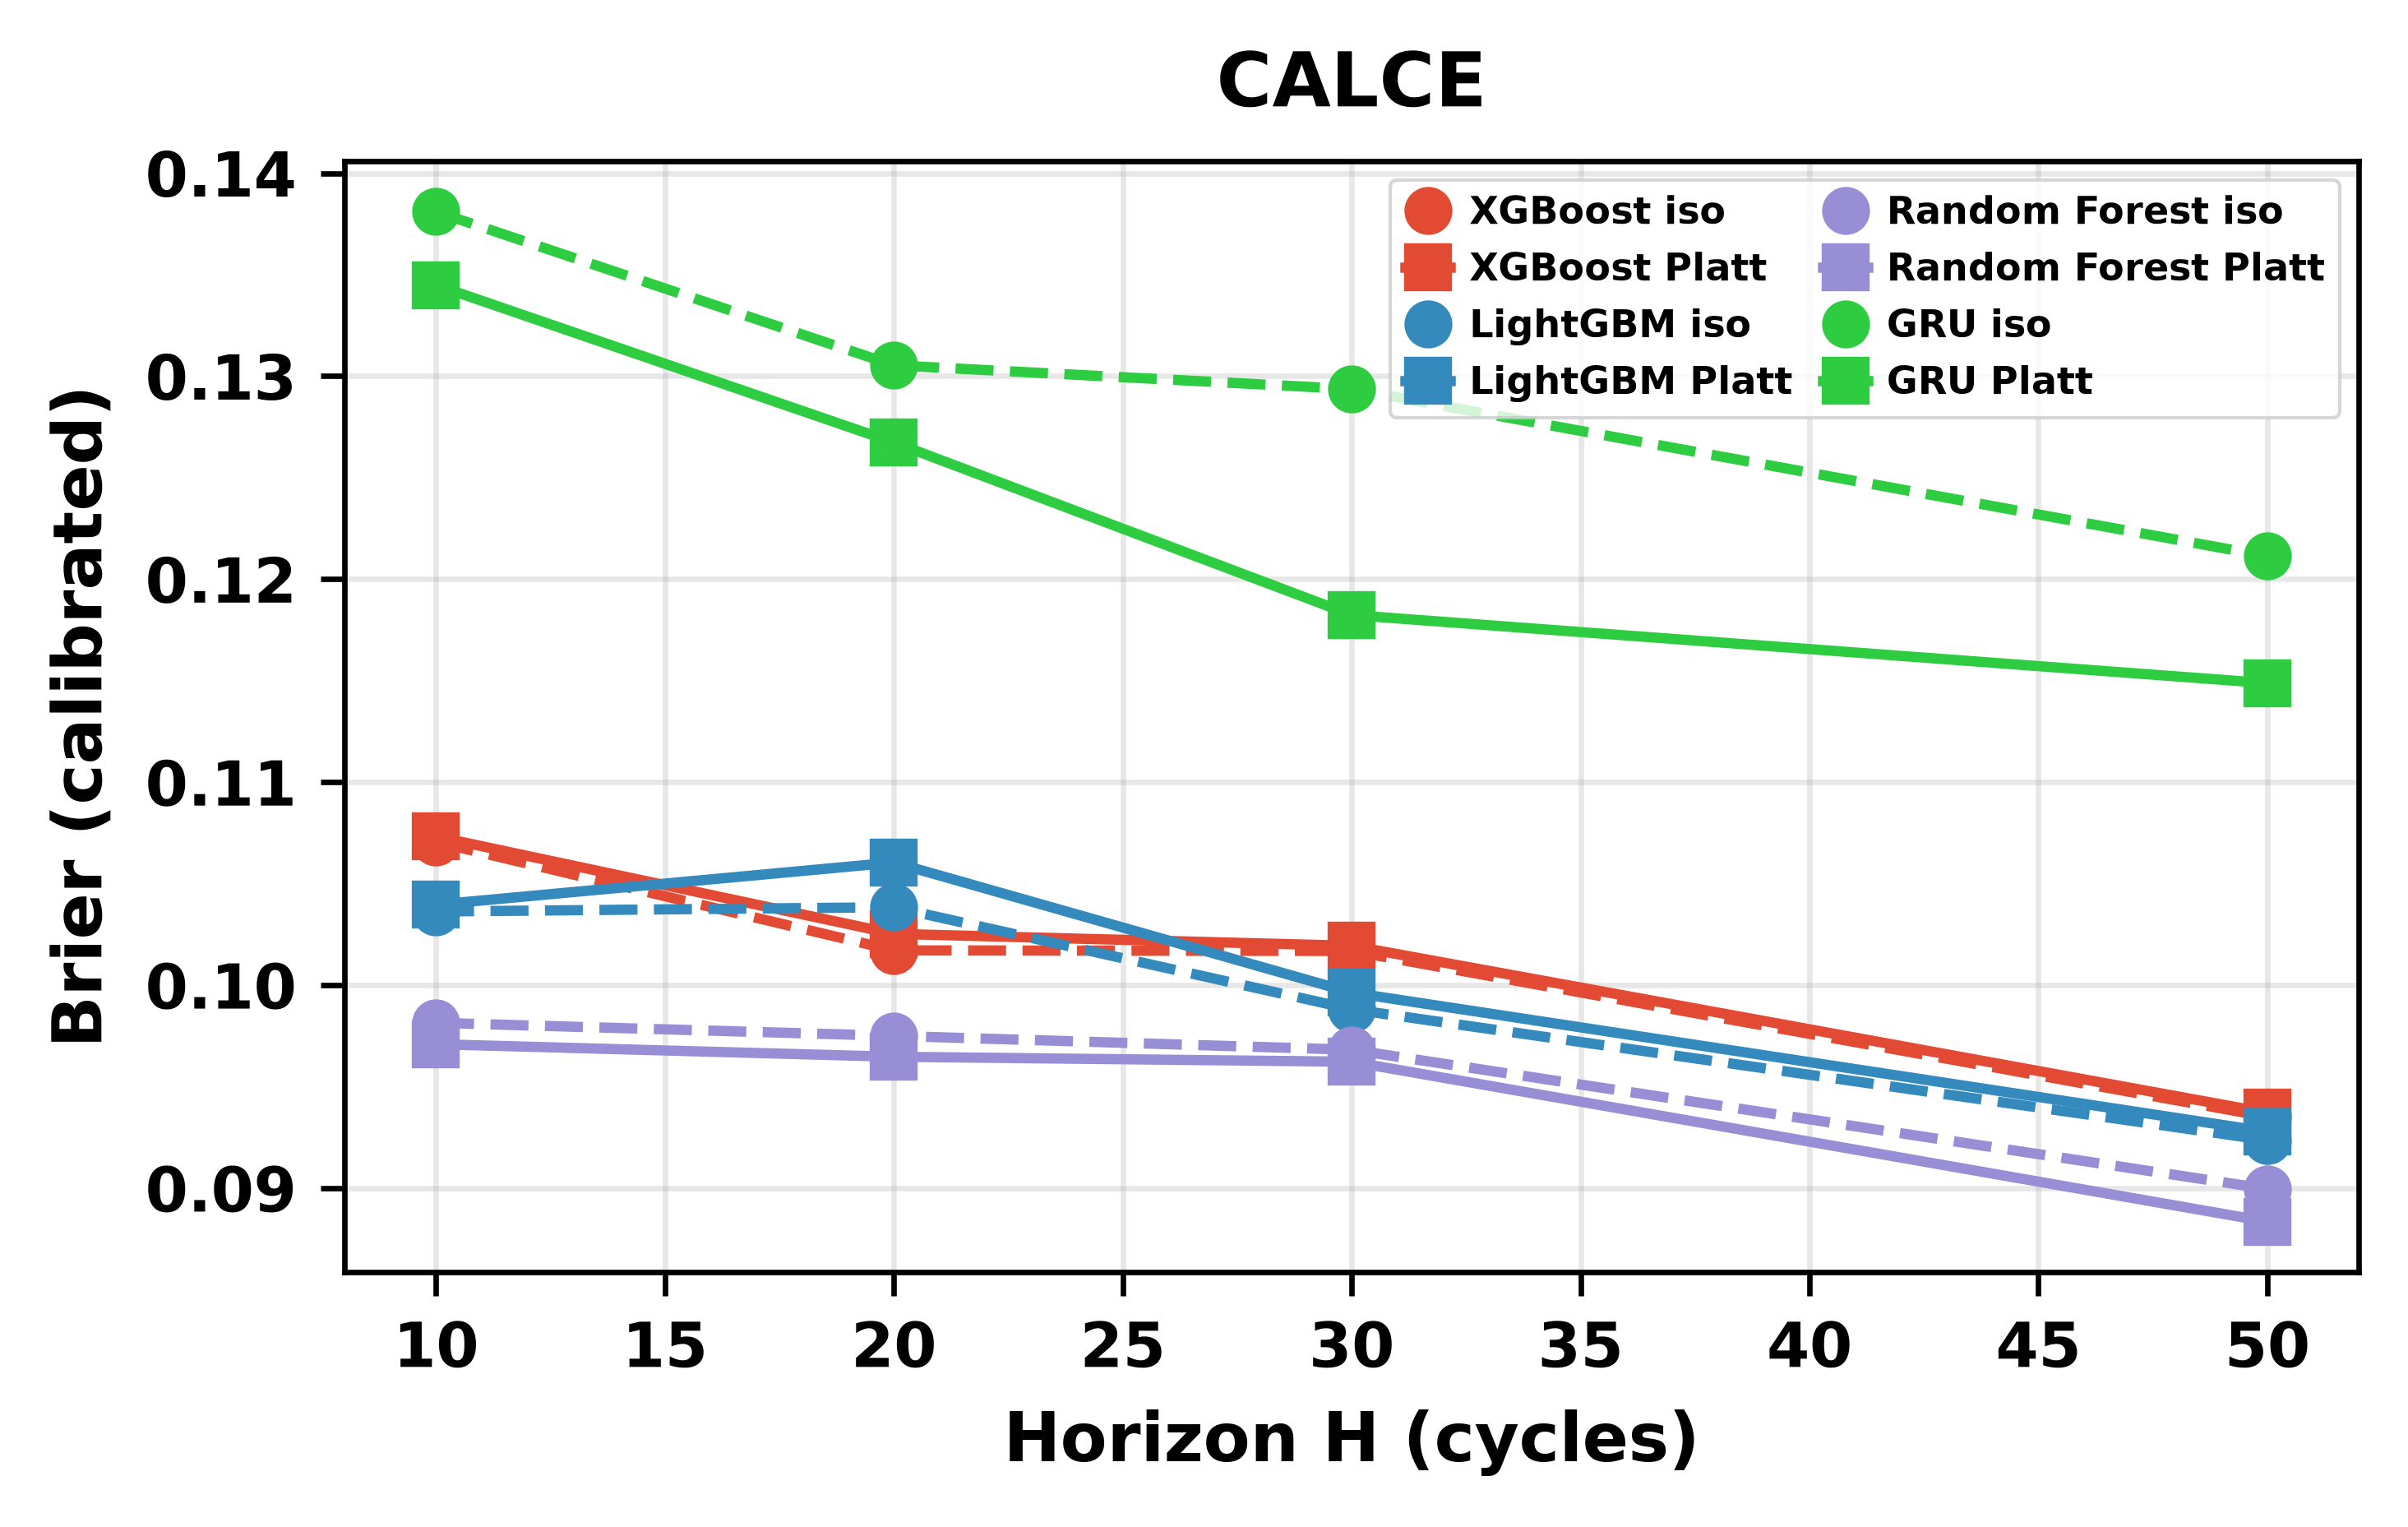
\includegraphics[width=\columnwidth]{Fig02b_Calibration_CALCE.png}
\caption{Calibration curves on CALCE at $H{=}20$: raw, Platt, isotonic, and temperature-scaled scores against the observed failure frequency.}
\label{fig:calcalce}
\end{figure}

\begin{figure}[!t]
\centering
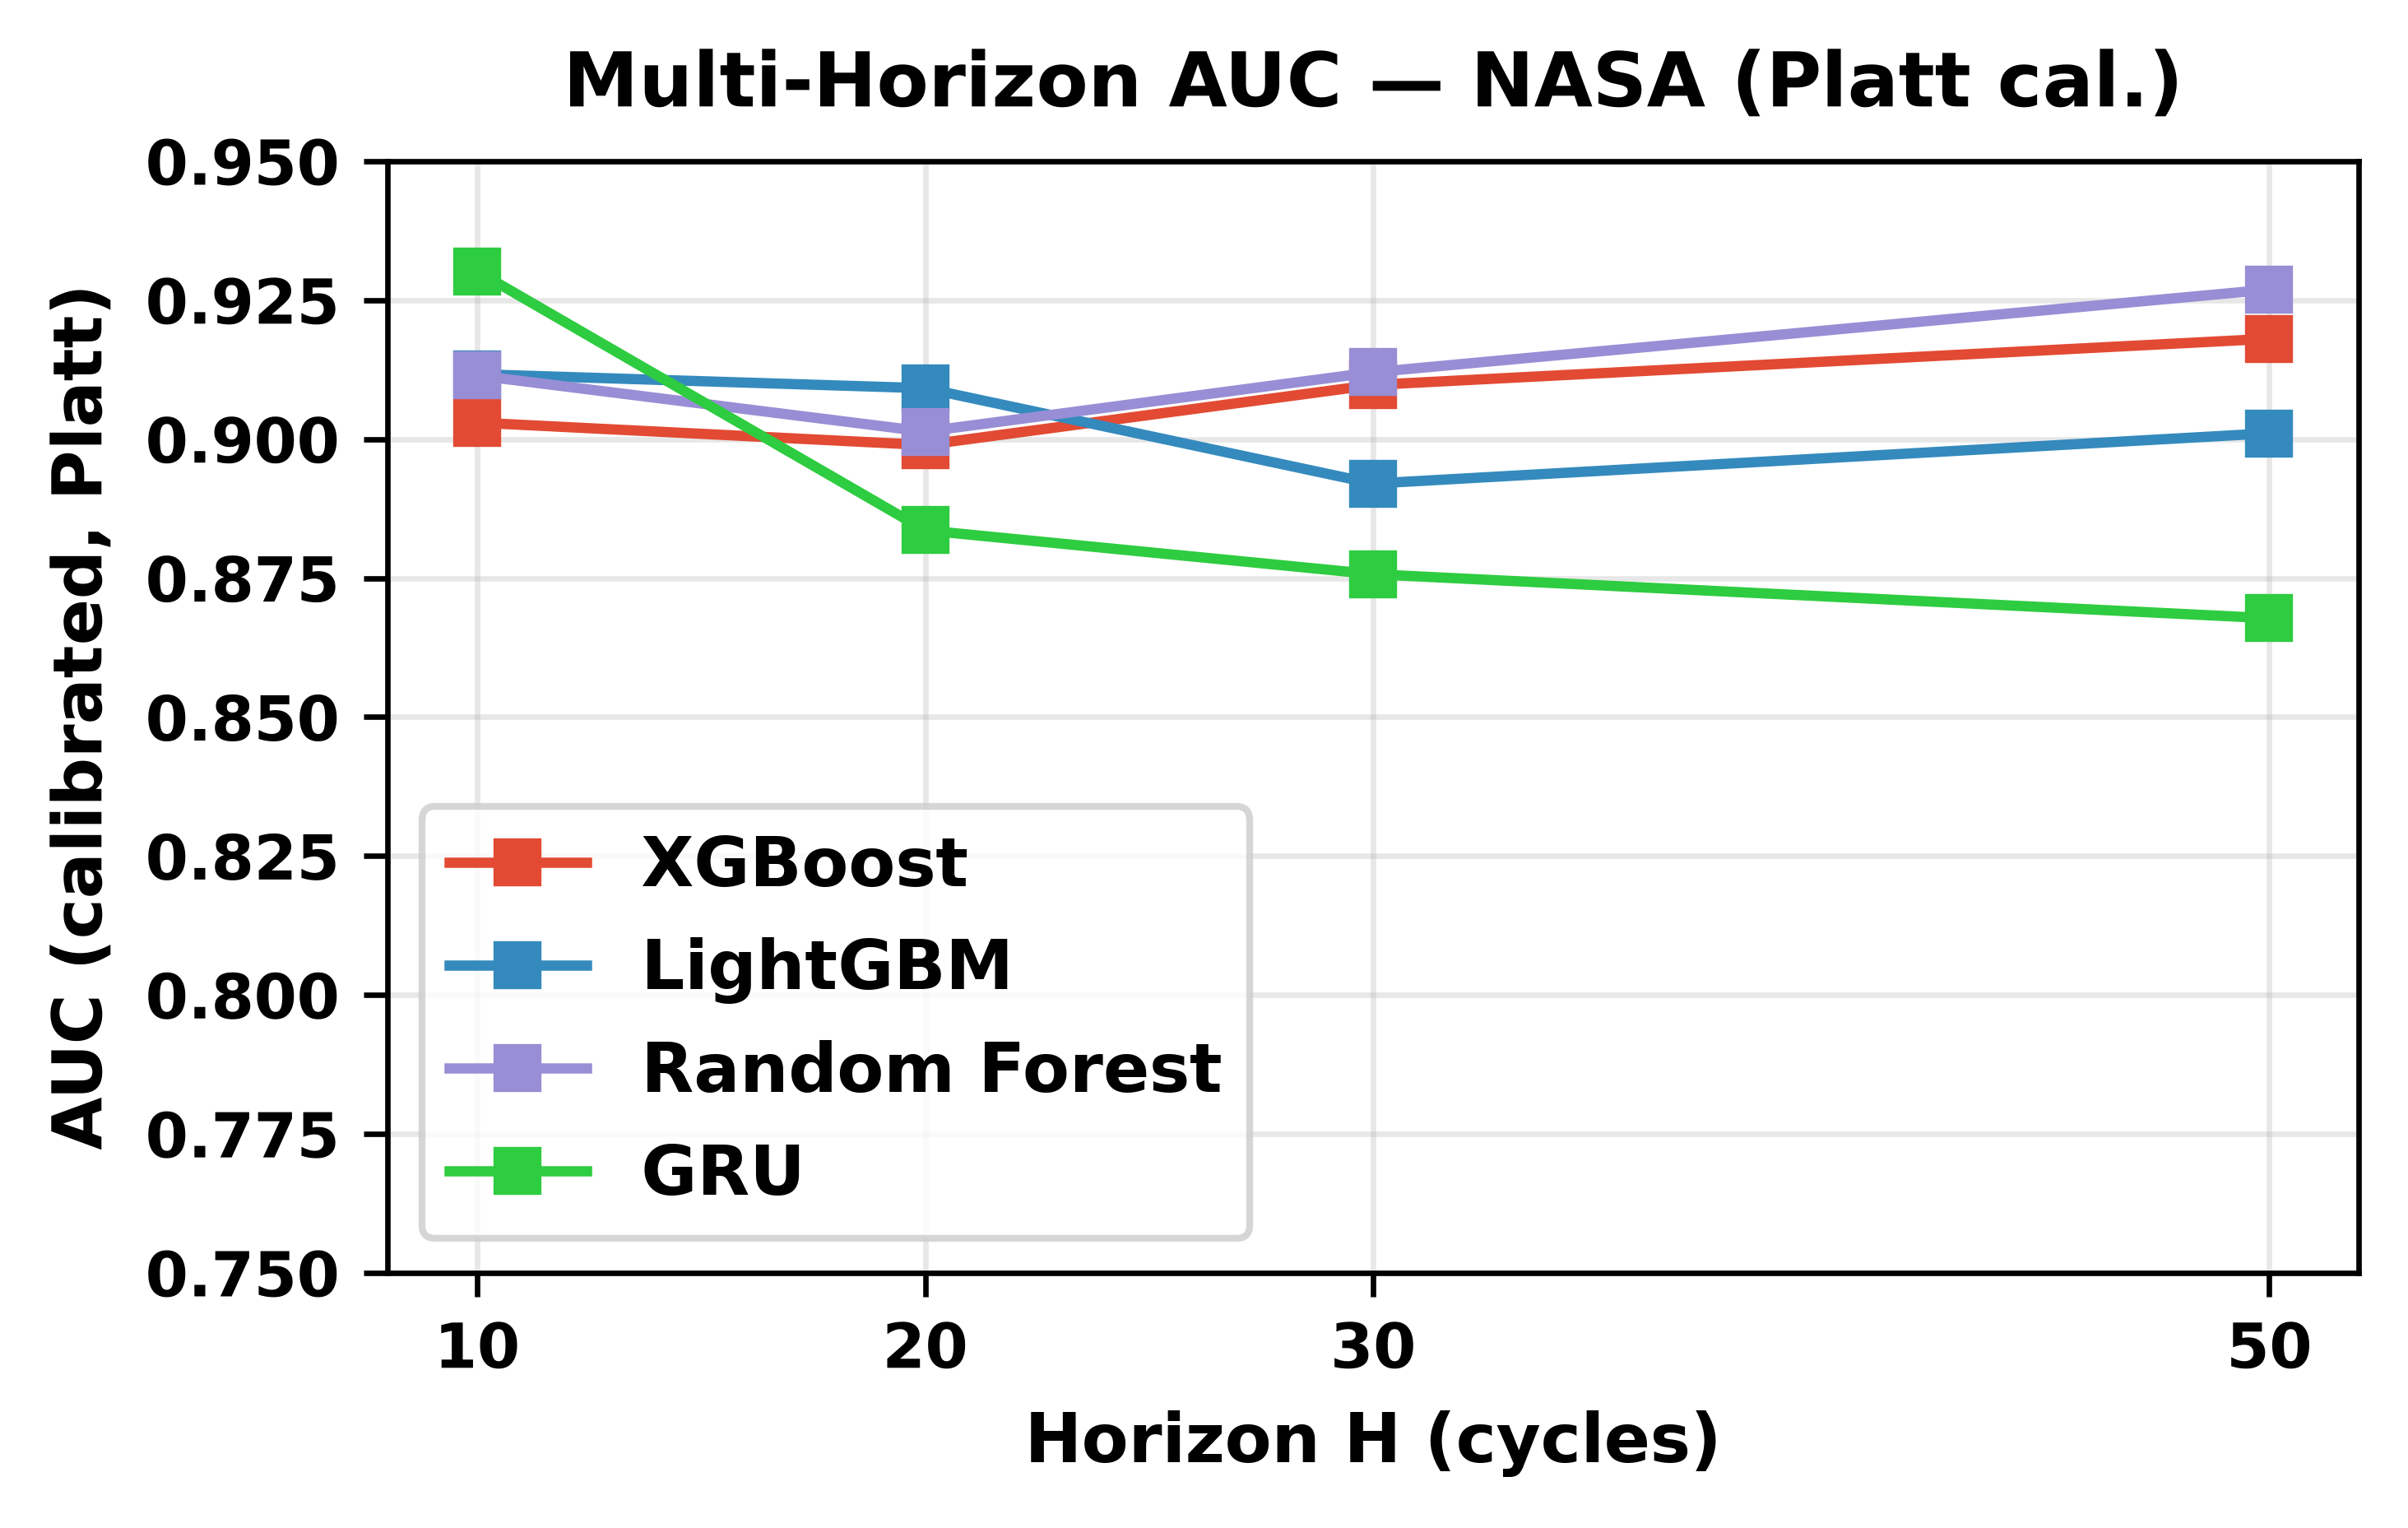
\includegraphics[width=\columnwidth]{Fig05_MultiHorizon_AUC.png}
\caption{Multi-horizon pooled AUC for the tree ensembles across $H\in\{10,20,30,50\}$: within-dataset stability against transfer degradation.}
\label{fig:multihorizon}
\end{figure}

\begin{figure}[!t]
\centering
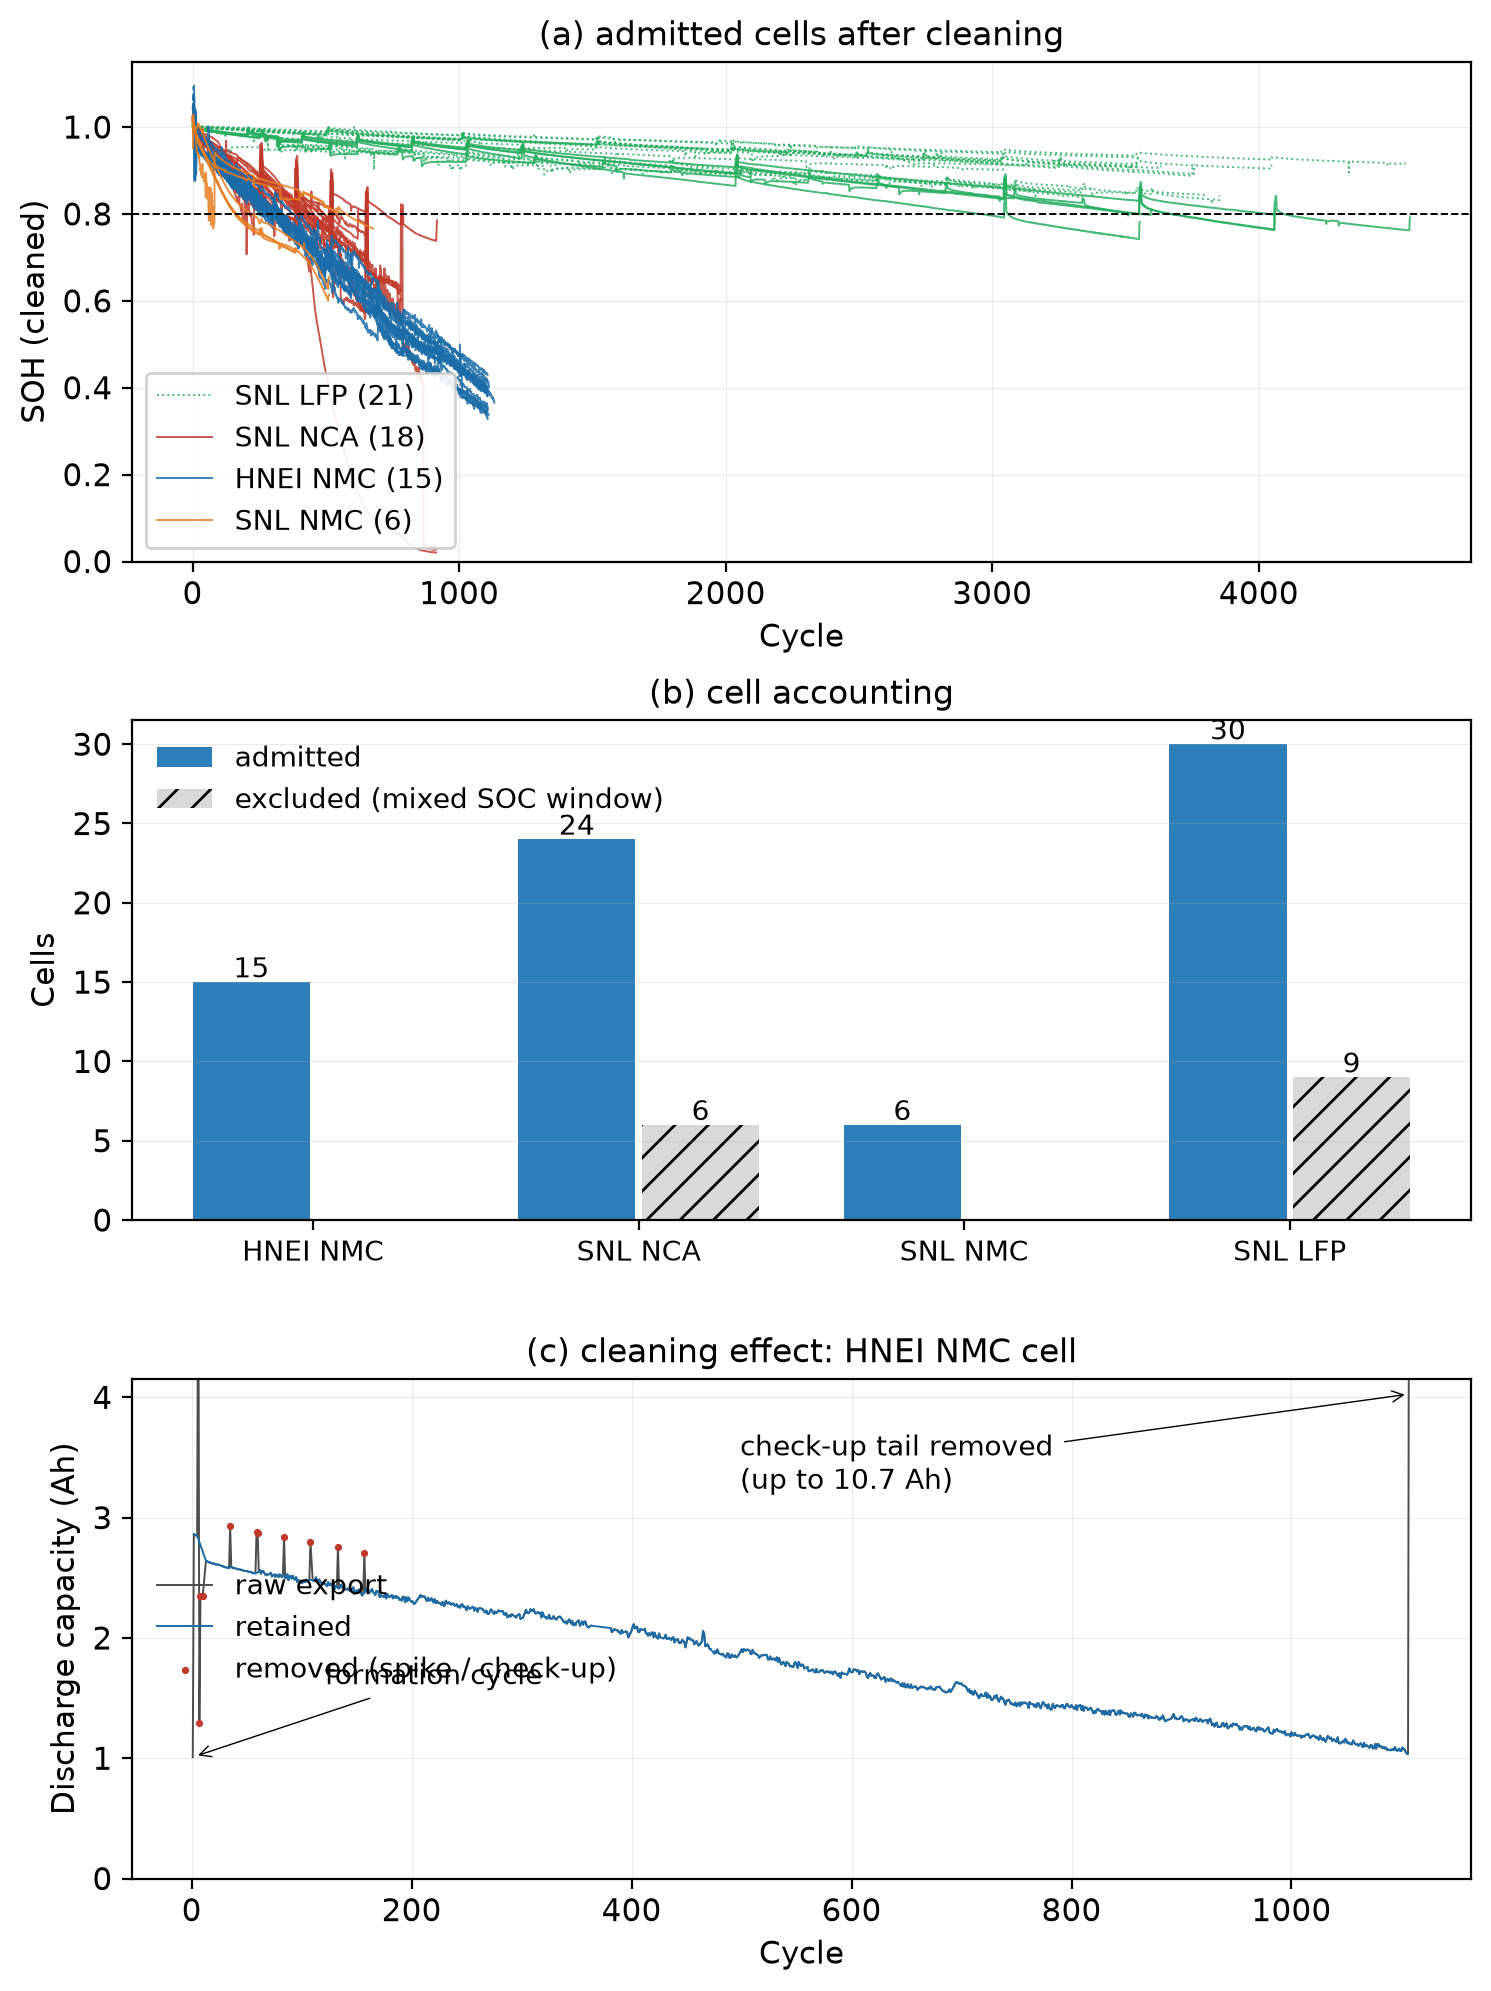
\includegraphics[width=\columnwidth]{fig_ba_quality.png}
\caption{Data audit of the Battery Archive groups after the pre-registered cleaning rule (formation-cycle drop, Hampel despiking, level-shift truncation, voltage validity, minimum 20 usable cycles): (a) admitted-cell capacity traces with the 80\% end-of-life criterion; (b) retained versus excluded cycles per group; (c) recorded exclusion reasons. Of 75 downloaded cells, 60 are admitted and 15 are excluded for exactly one recorded reason.}
\label{fig:baquality}
\end{figure}

\begin{figure}[!t]
\centering
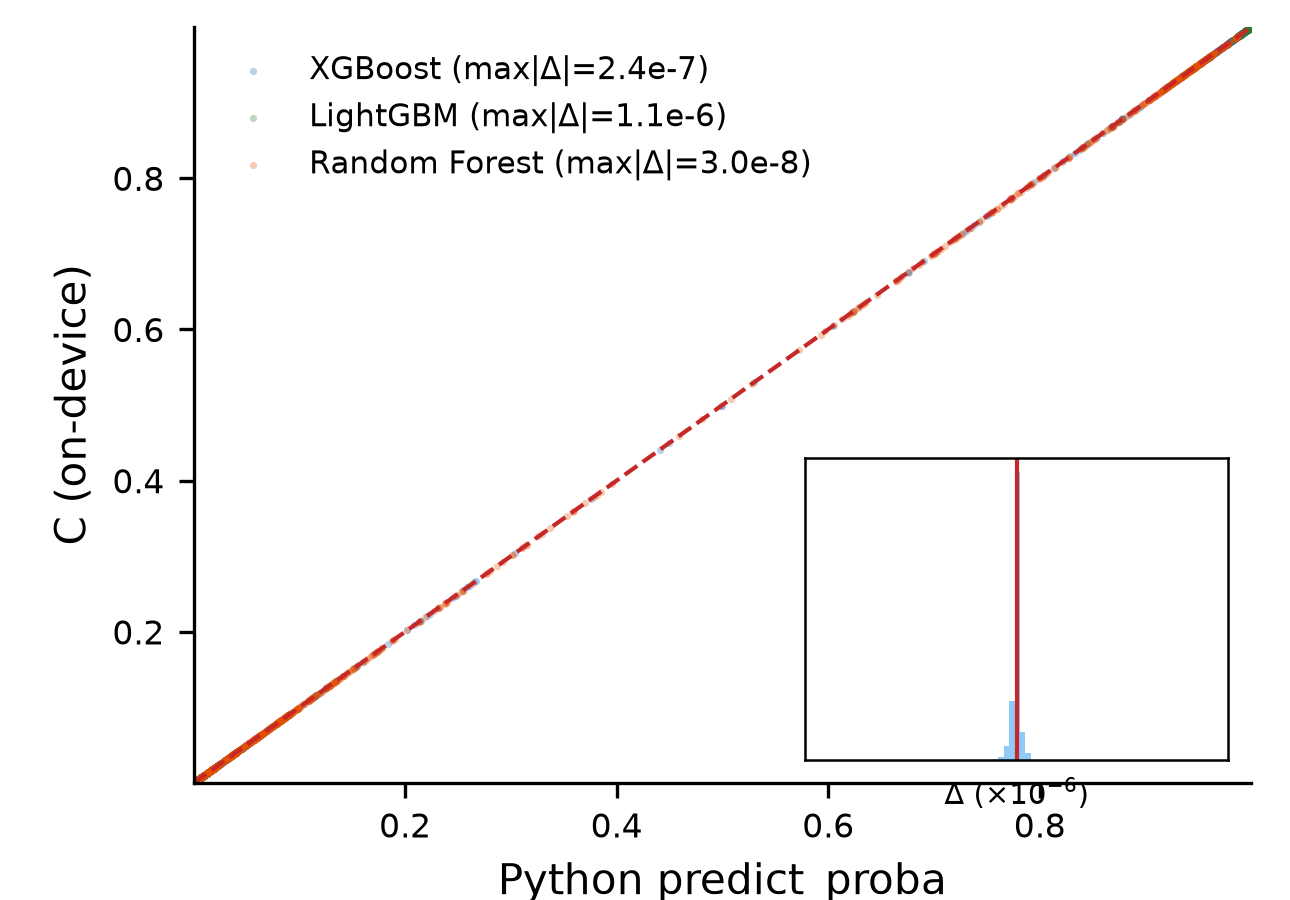
\includegraphics[width=\columnwidth]{fig_py_c_agreement.png}
\caption{On-device C engine predictions versus Python \texttt{predict\_proba()} over all 1 028 rows and three models (agreement scatter on the identity line, inset residual histogram of C minus Python in units of $10^{-6}$). Maximum absolute errors are $2.4\times10^{-7}$ (XGBoost), $1.1\times10^{-6}$ (LightGBM), and $3.0\times10^{-8}$ (Random Forest).}
\label{fig:pyc}
\end{figure}

\begin{figure}[!t]
\centering
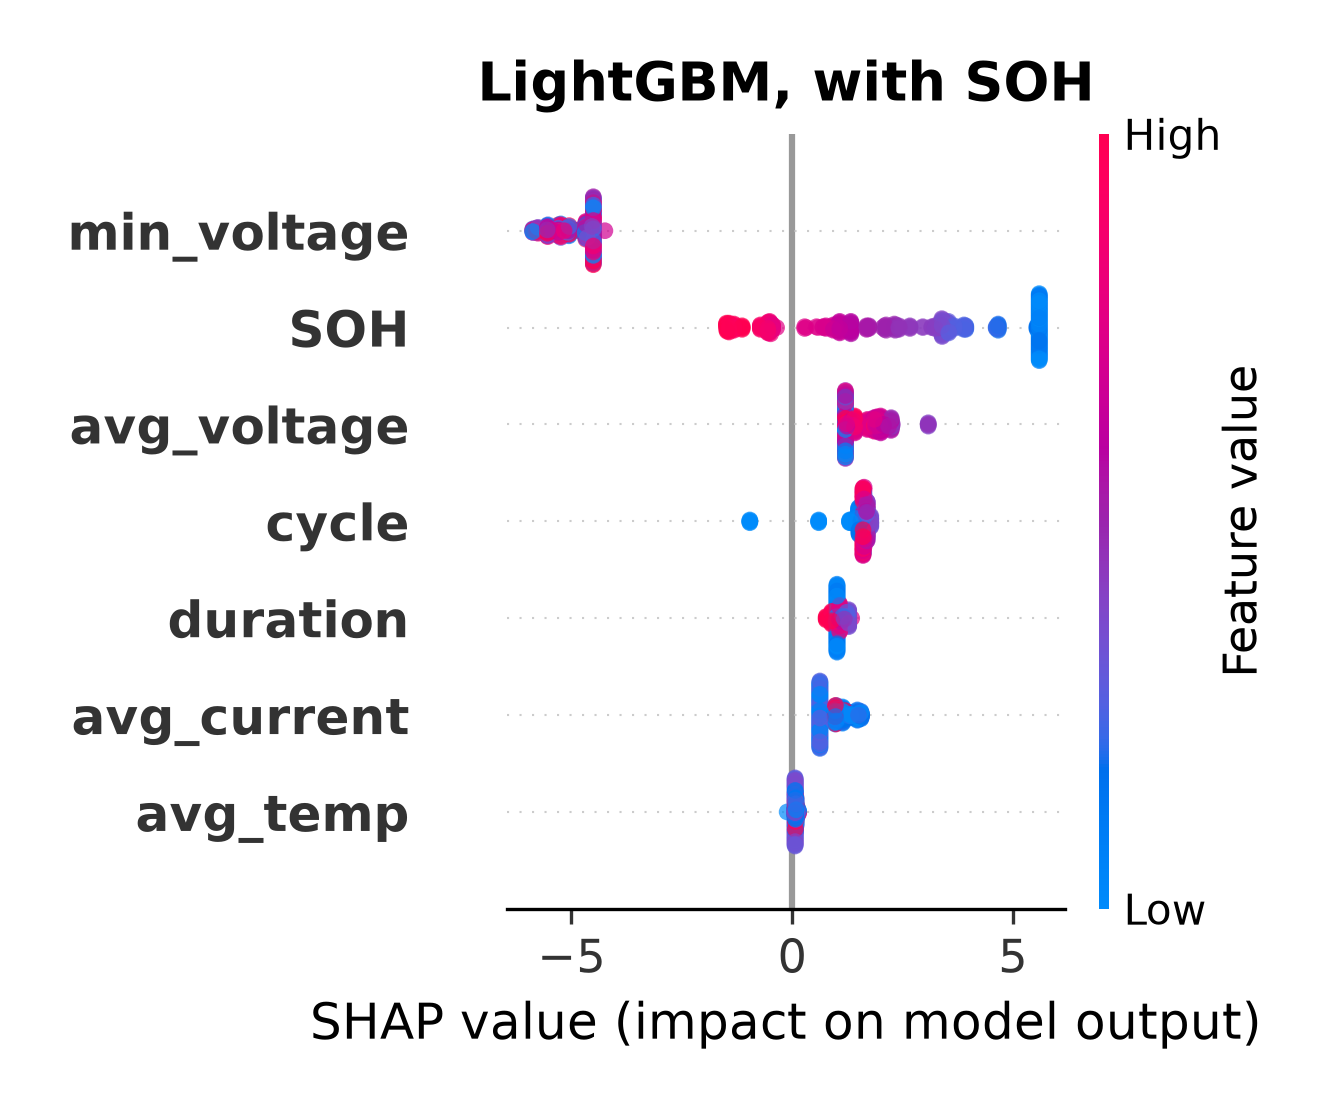
\includegraphics[width=\columnwidth]{Fig06b_LightGBM_SHAP.png}
\caption{SHAP feature importance for LightGBM in NASA-to-Oxford transfer at $H{=}20$, with SOH. SOH dominates by a wide margin (cf.\ main manuscript, Fig.\ 5).}
\label{fig:shap_lgbm}
\end{figure}

\begin{figure}[!t]
\centering
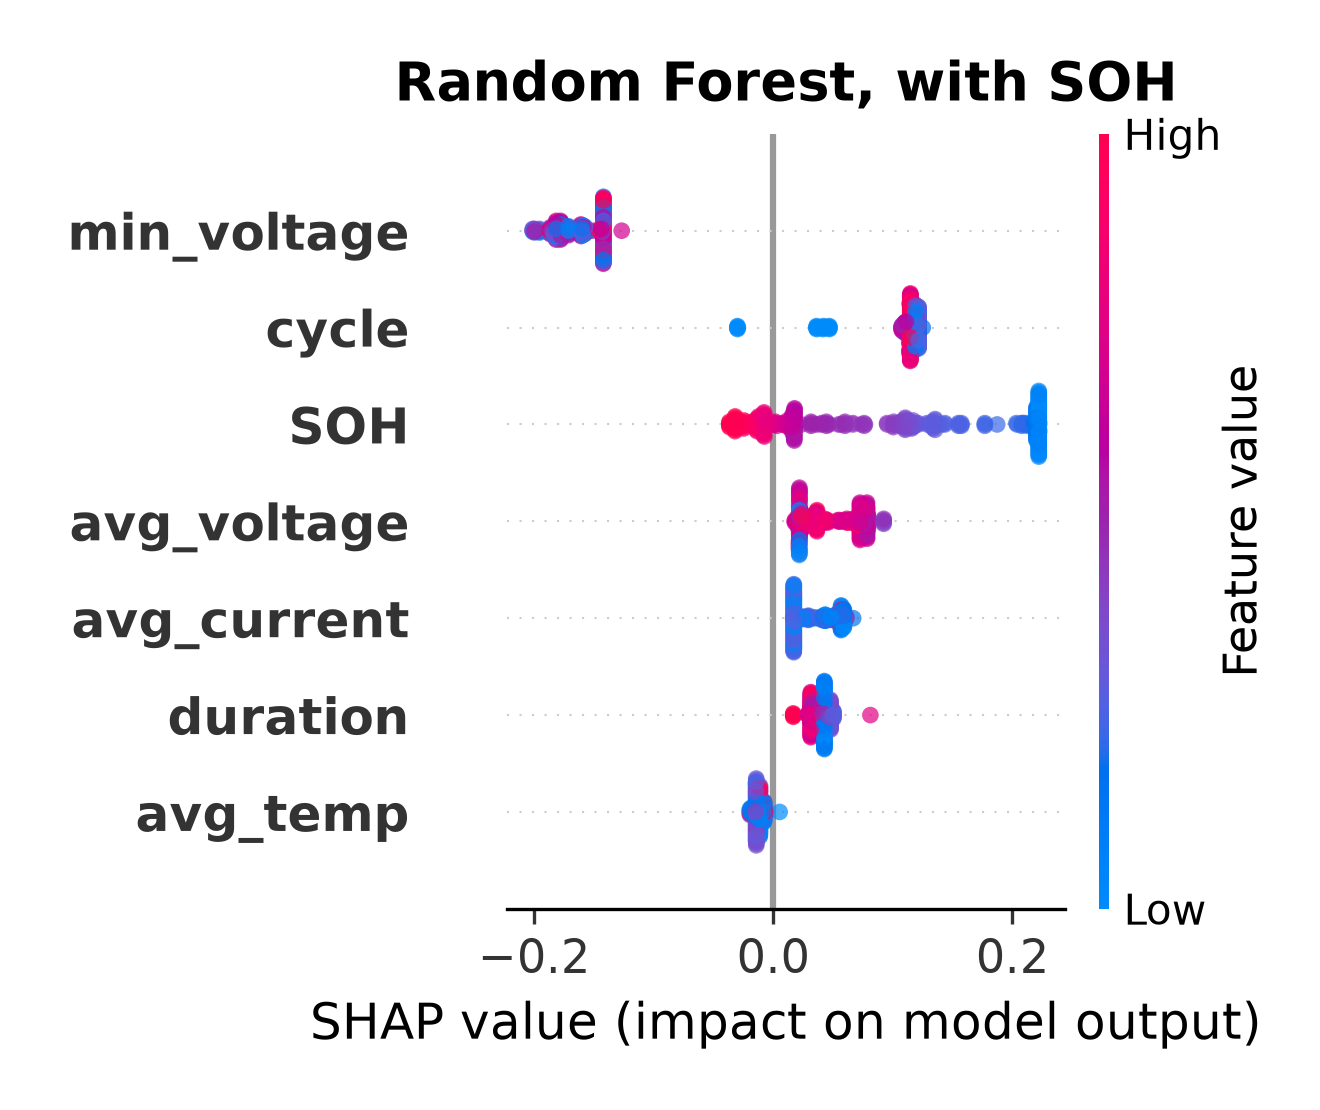
\includegraphics[width=\columnwidth]{Fig06c_RandomForest_SHAP.png}
\caption{SHAP feature importance for Random Forest in NASA-to-Oxford transfer at $H{=}20$, with SOH. SOH dominates by a wide margin.}
\label{fig:shap_rf}
\end{figure}

\begin{figure}[!t]
\centering
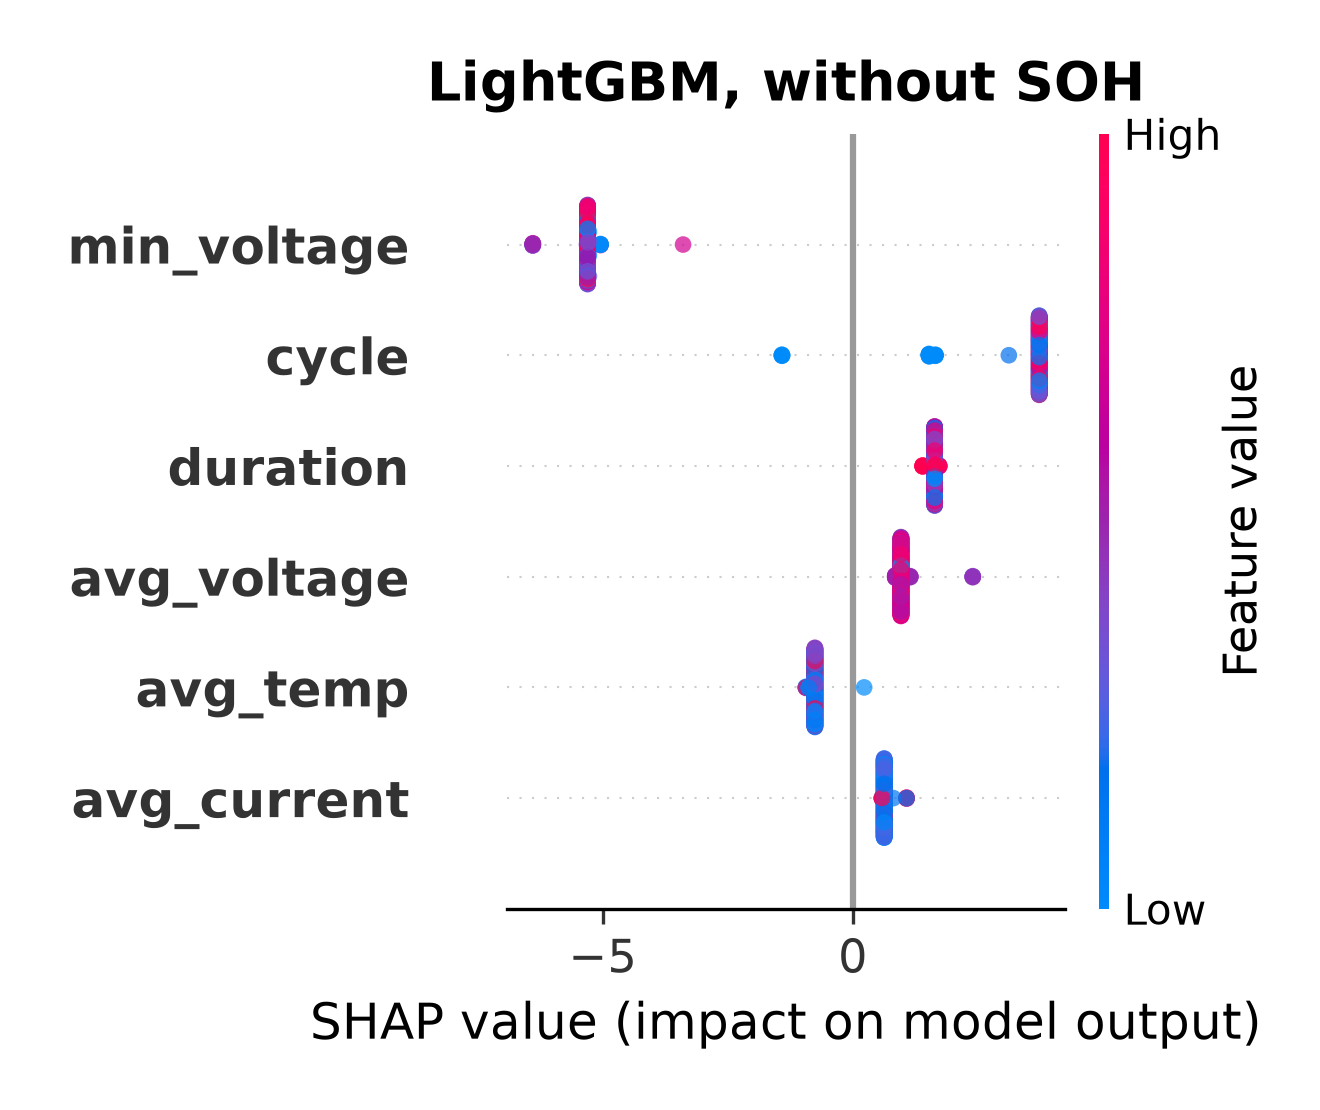
\includegraphics[width=\columnwidth]{Fig06e_LightGBM_SHAP_noSOH.png}
\caption{SHAP feature importance for LightGBM in NASA-to-Oxford transfer at $H{=}20$, without SOH. All features collapse to near-zero spread.}
\label{fig:shap_nolgbm}
\end{figure}

\begin{figure}[!t]
\centering
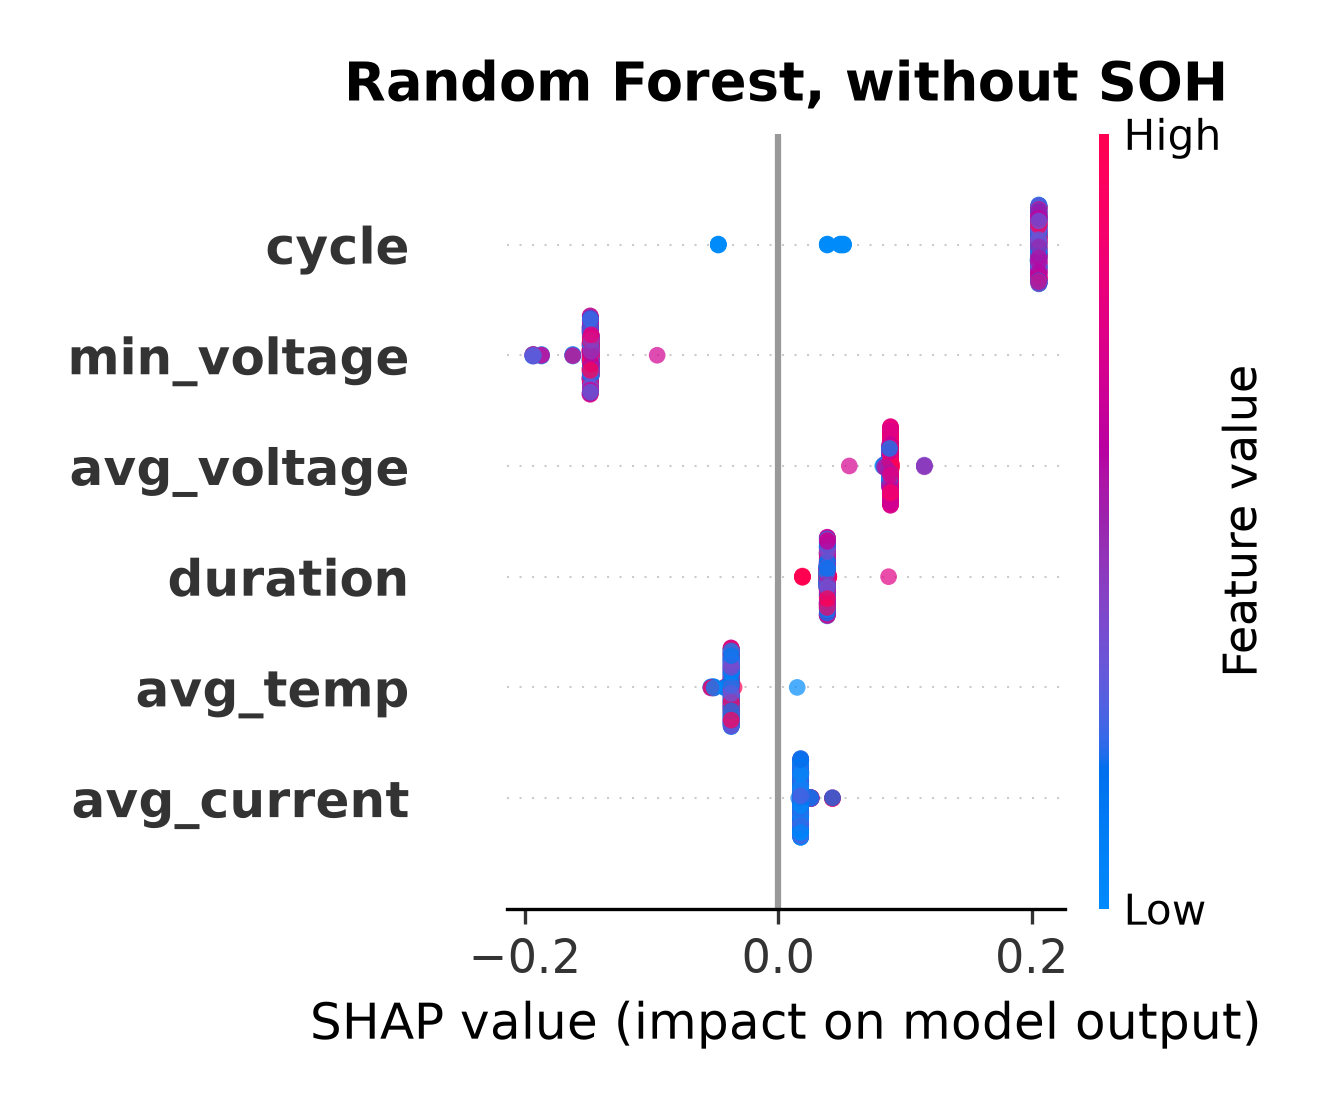
\includegraphics[width=\columnwidth]{Fig06f_RandomForest_SHAP_noSOH.png}
\caption{SHAP feature importance for Random Forest in NASA-to-Oxford transfer at $H{=}20$, without SOH. All features collapse to near-zero spread.}
\label{fig:shap_norf}
\end{figure}

\begin{figure}[!t]
\centering
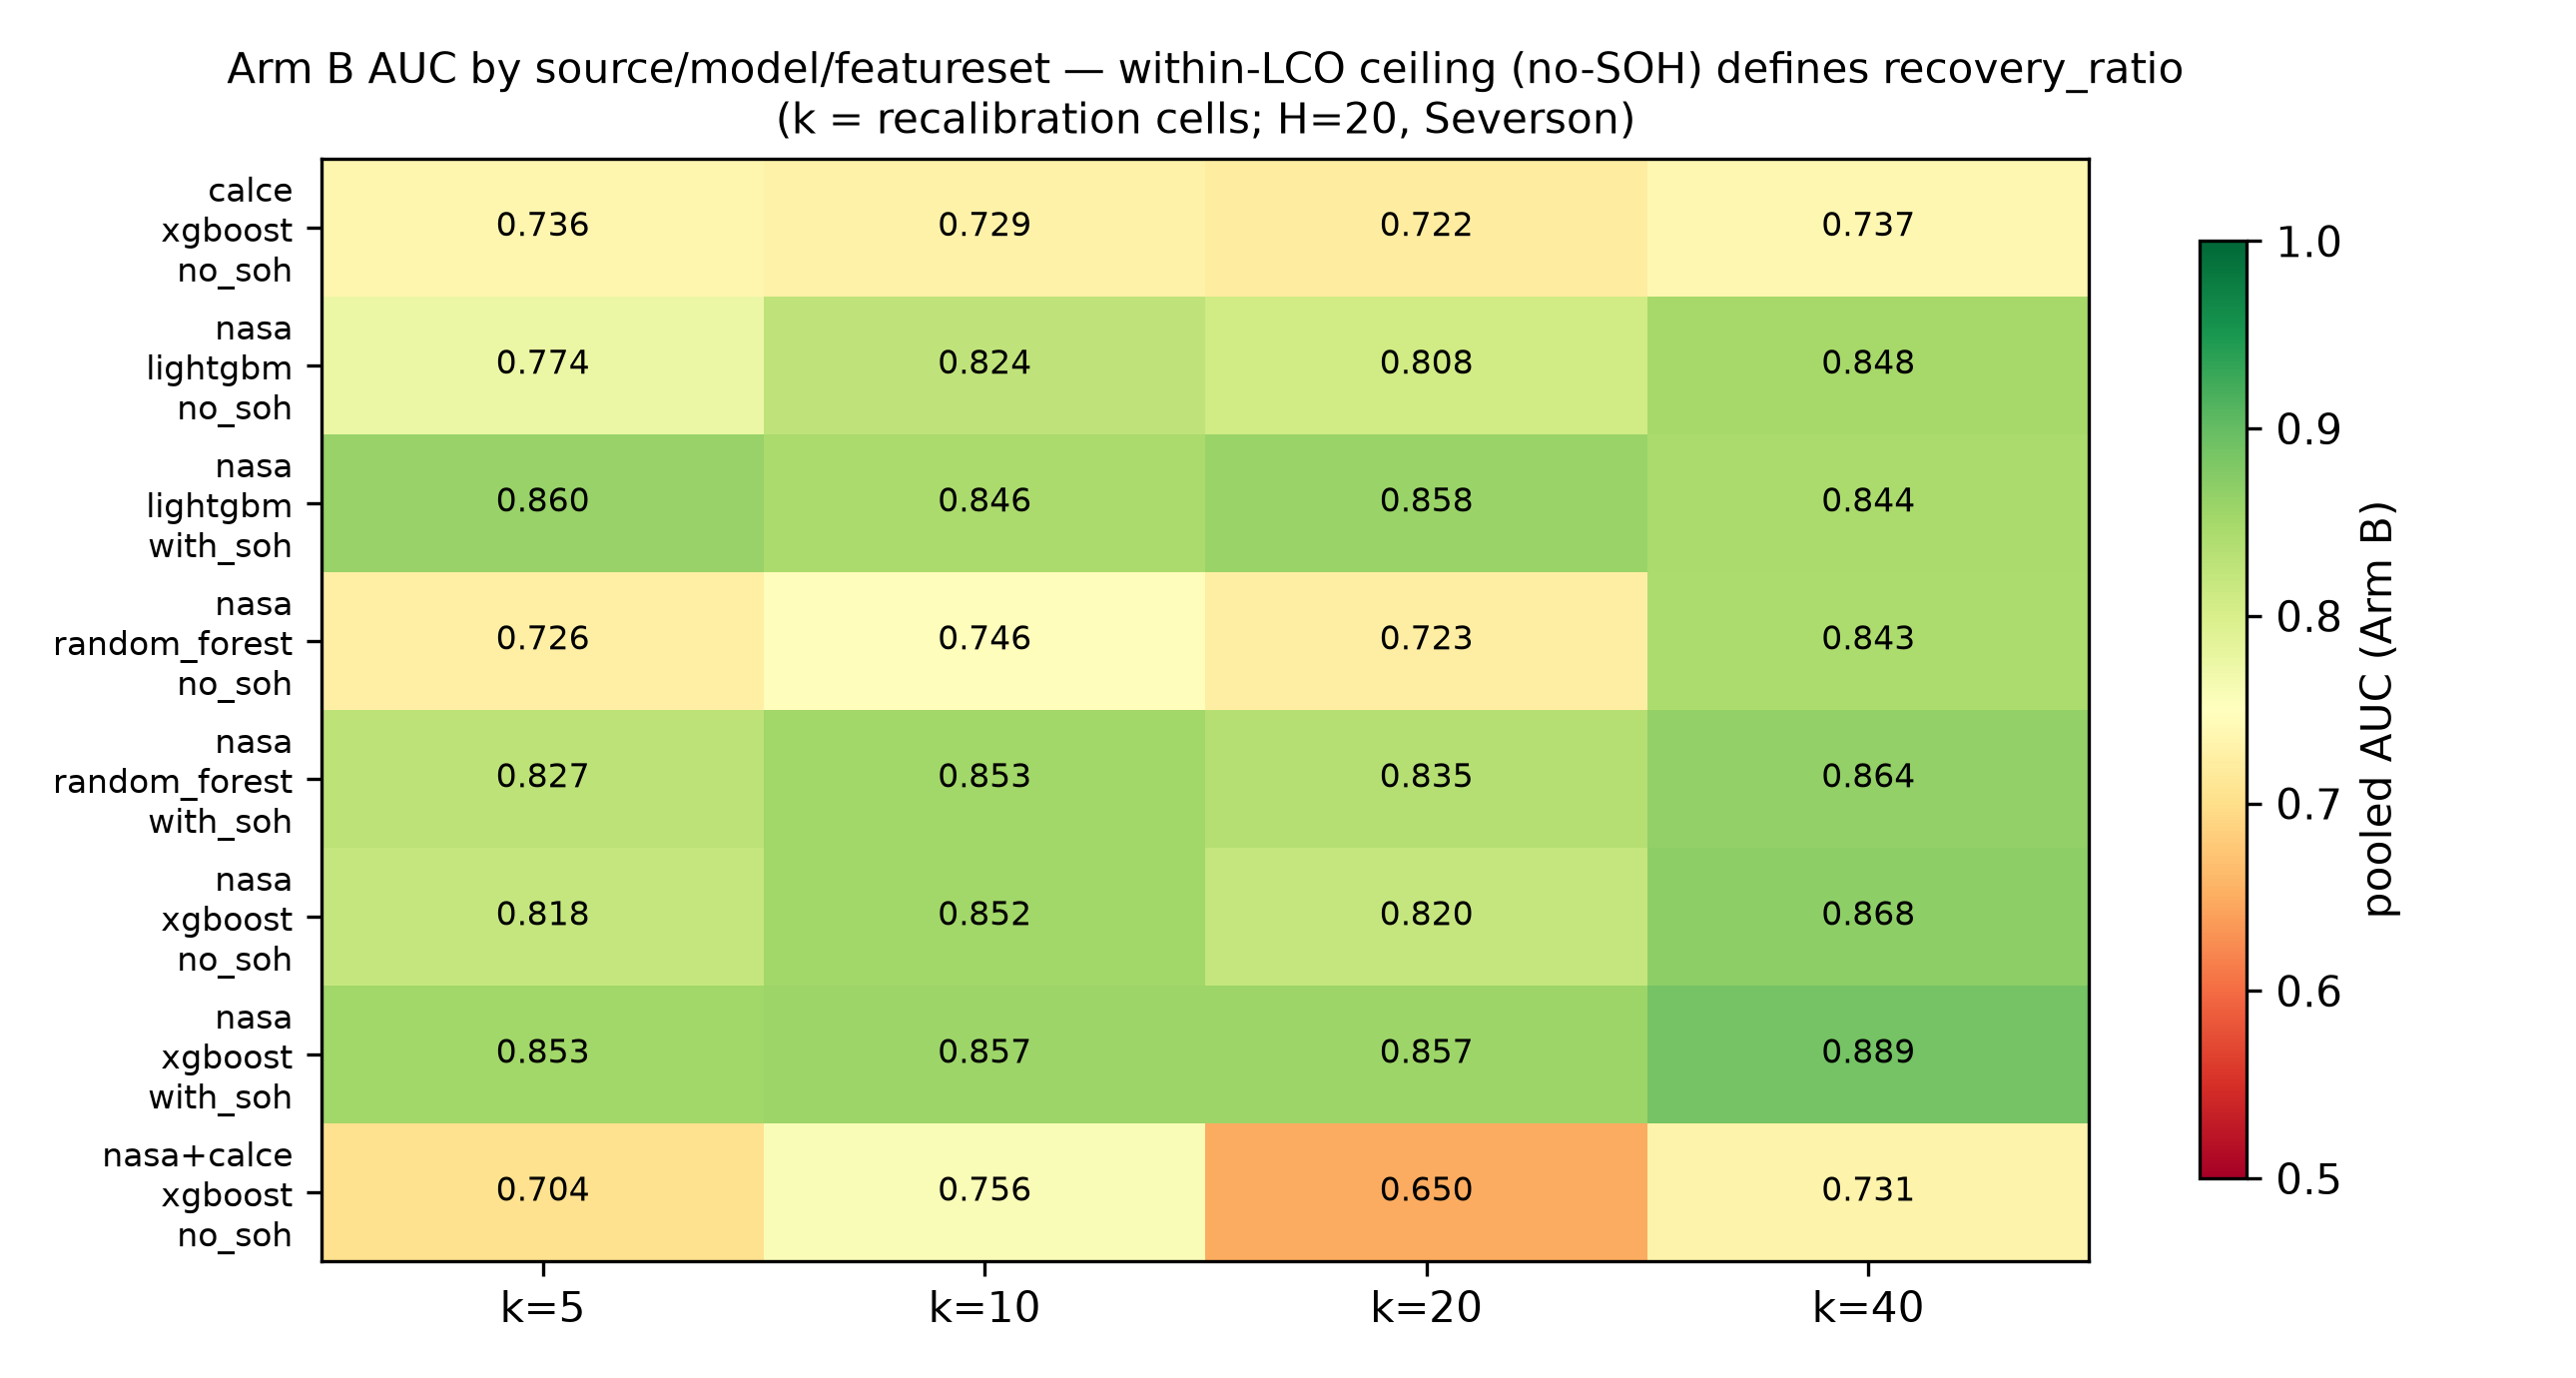
\includegraphics[width=\columnwidth]{fig_recal_heatmap.png}
\caption{Recalibration heatmap: calibration error across target-set sizes and calibrators for the Arm A protocol (main manuscript, Section III-H).}
\label{fig:recalheat}
\end{figure}

\begin{figure}[!t]
\centering
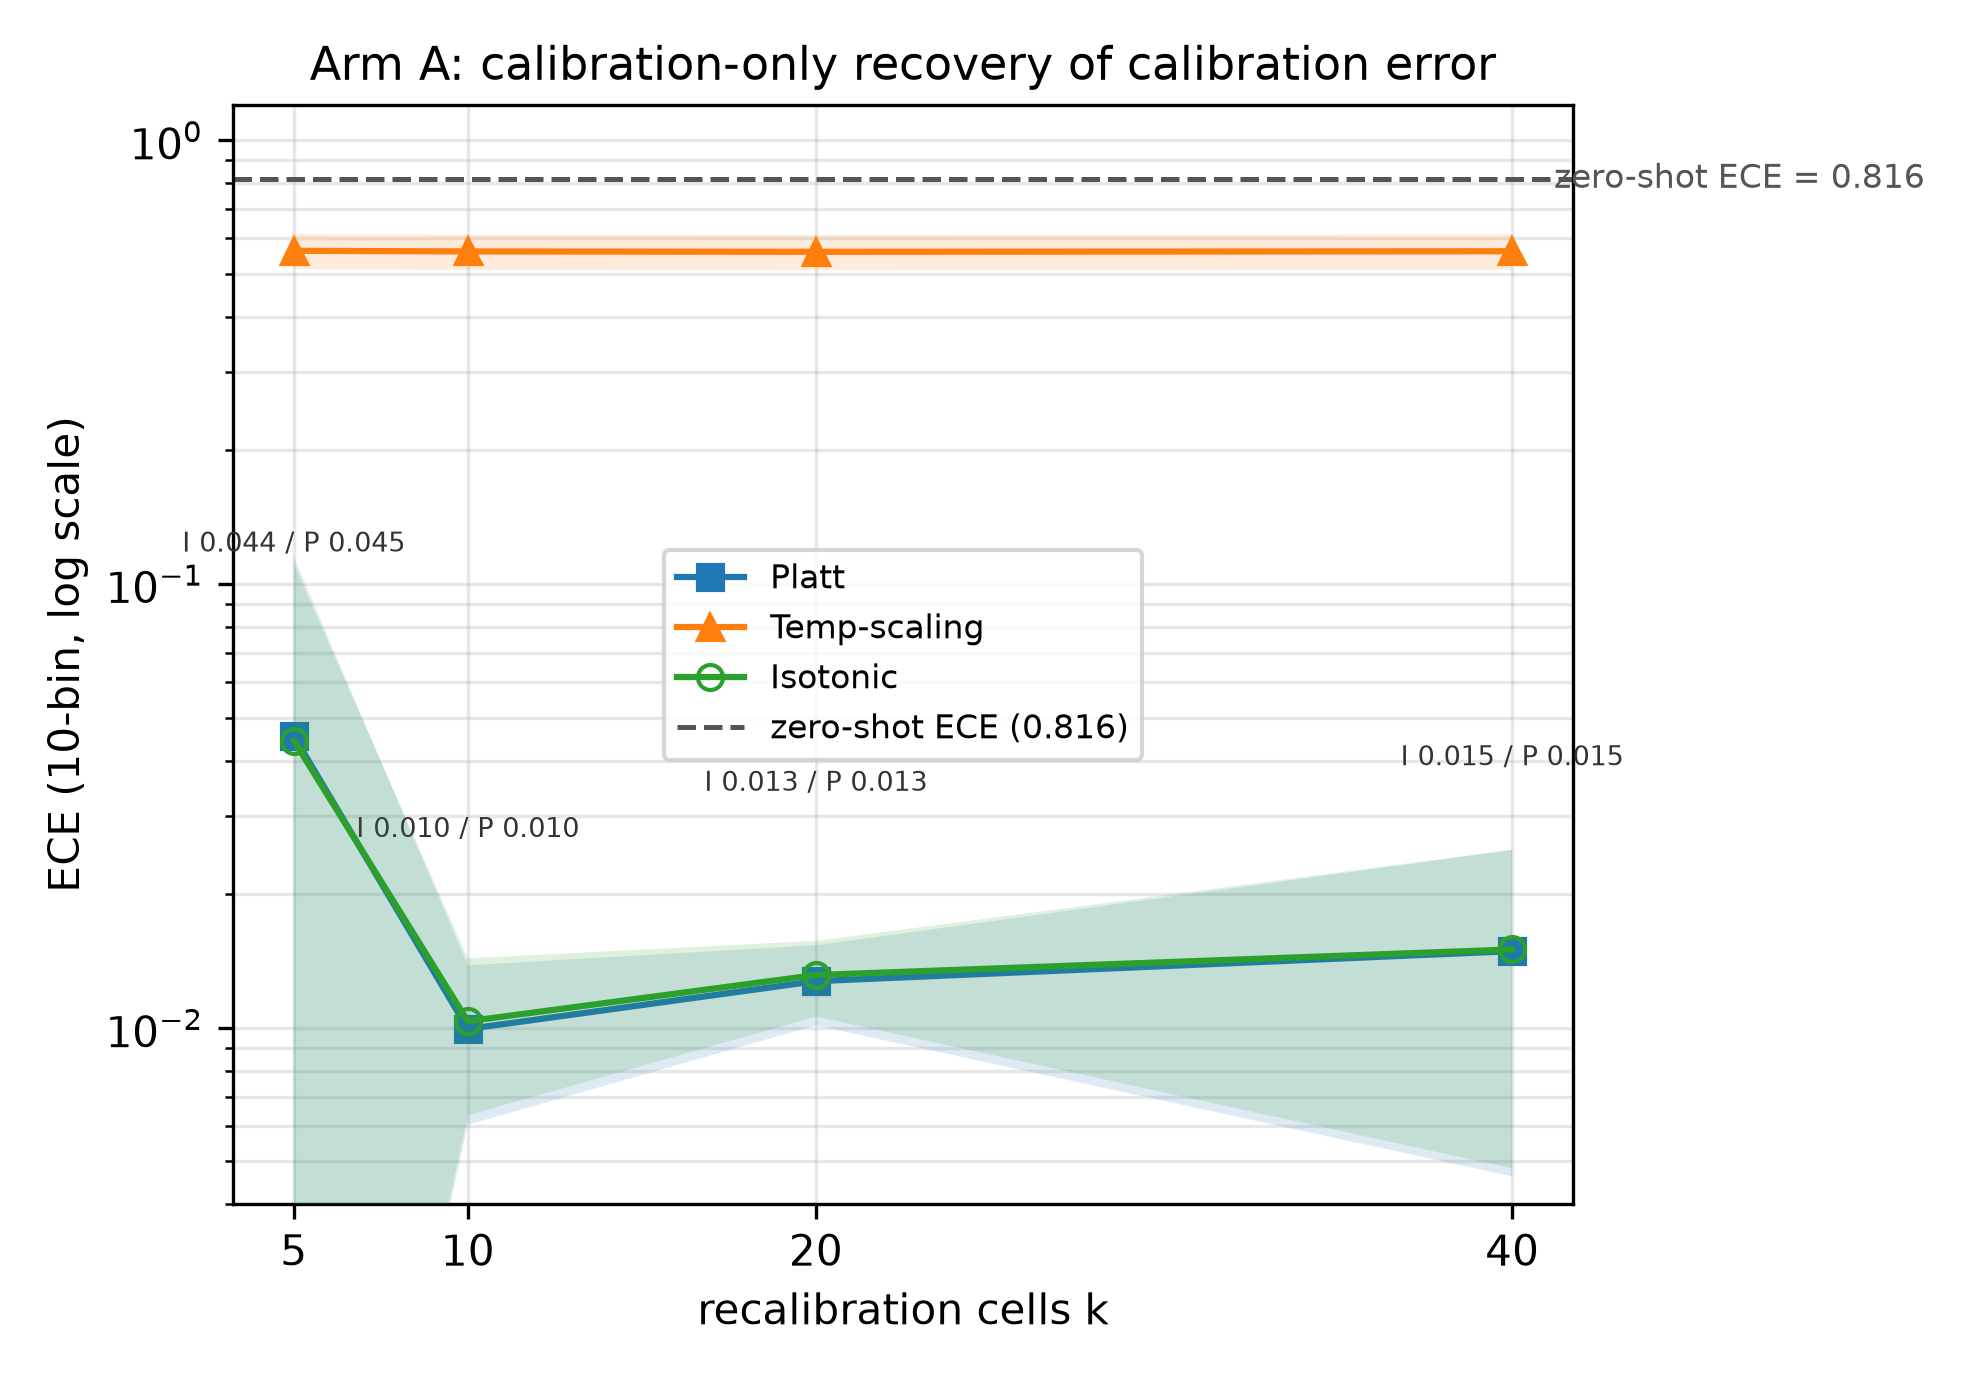
\includegraphics[width=\columnwidth]{fig_recal_ece_vs_k.png}
\caption{Arm A recalibration: expected calibration error versus number of labeled target cells $k$ on Severson without SOH.}
\label{fig:recalece}
\end{figure}

\begin{figure}[!t]
\centering
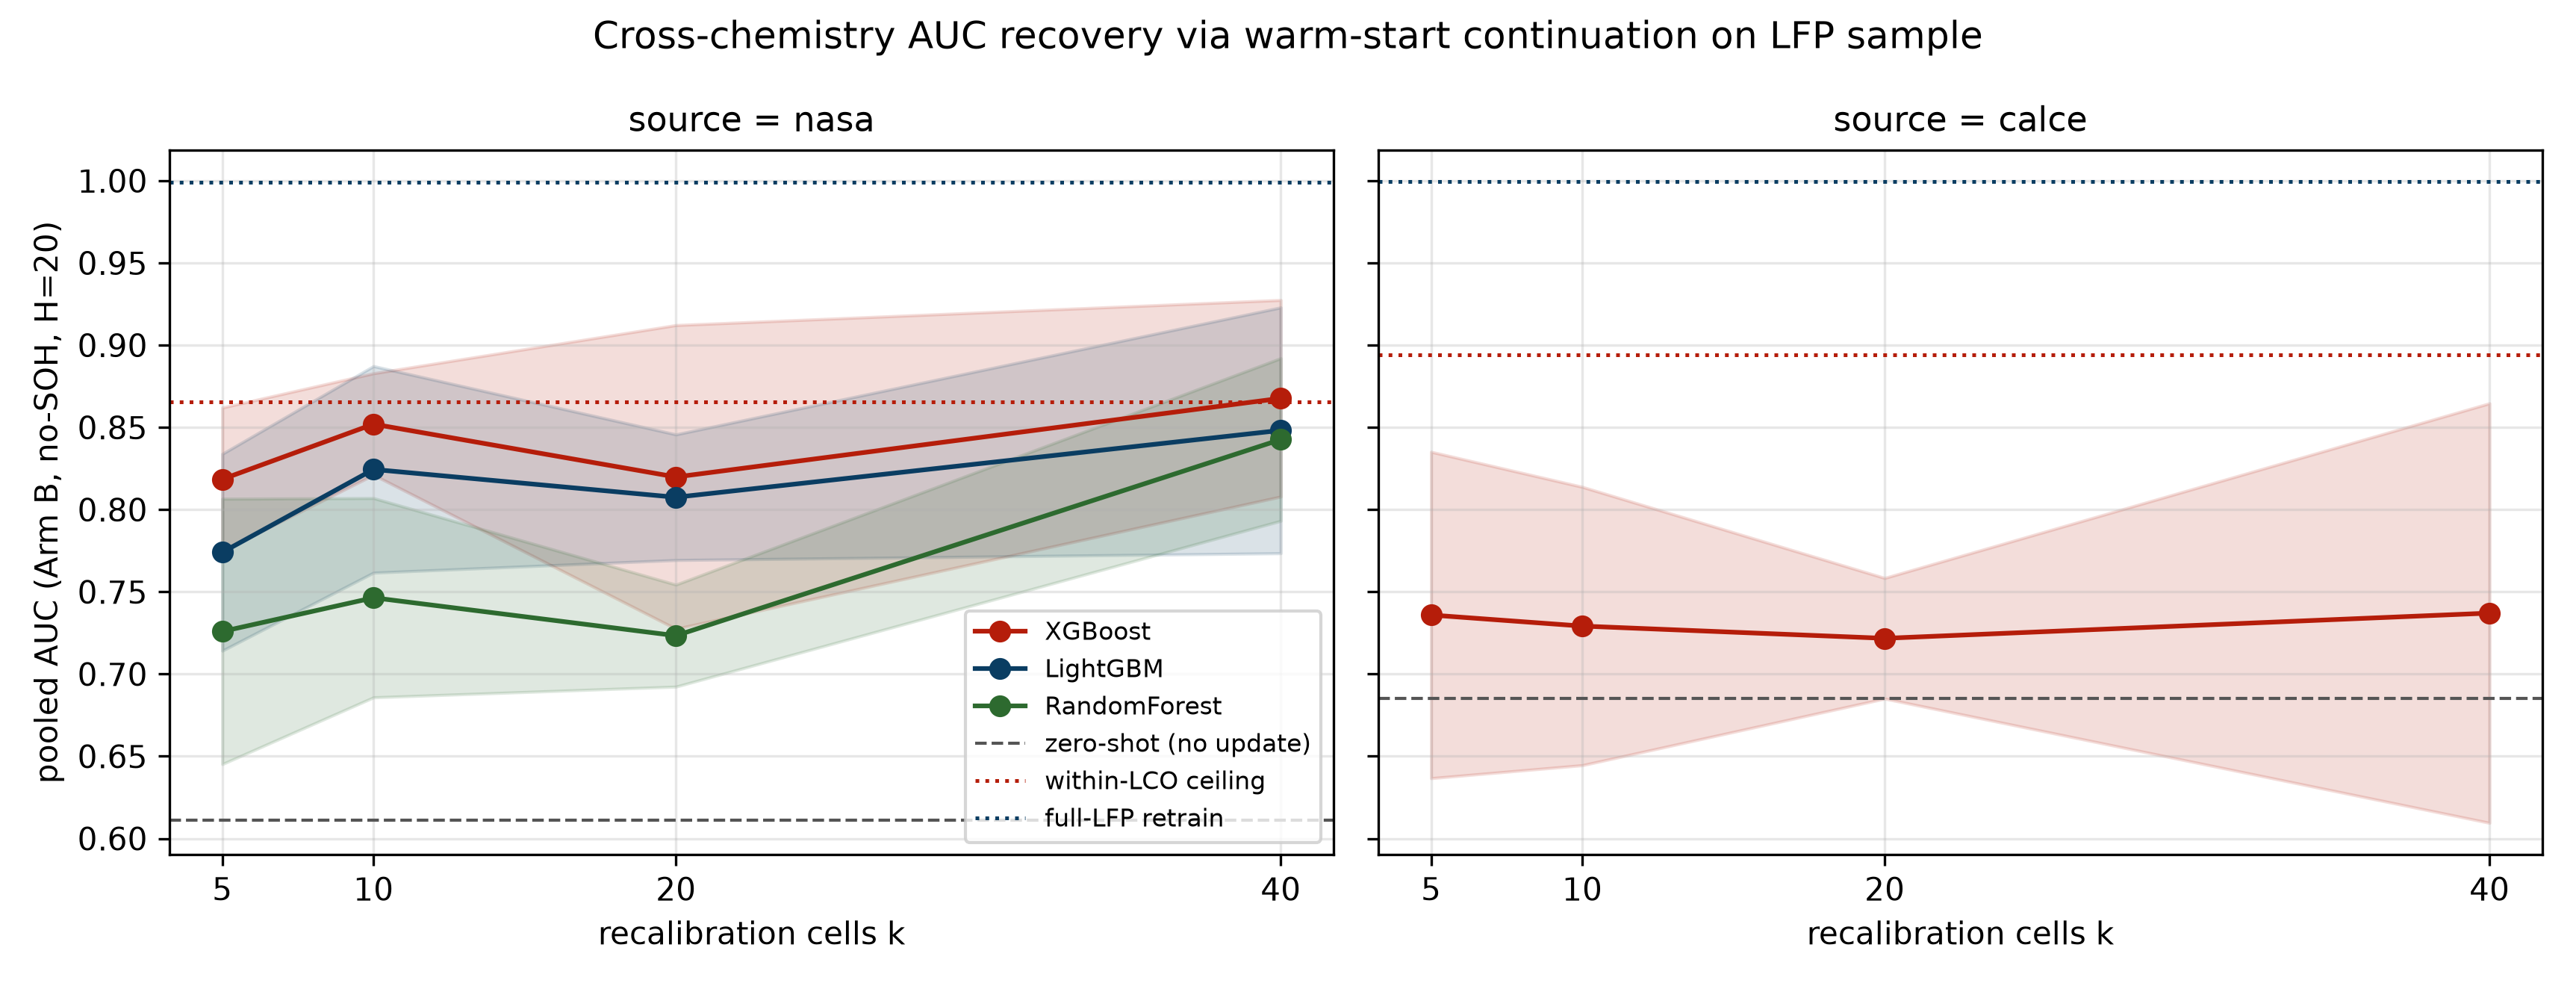
\includegraphics[width=\columnwidth]{fig_recal_auc_vs_k.png}
\caption{Arm A recalibration: pooled AUC versus number of labeled target cells $k$ on Severson without SOH --- calibration error is repaired; discrimination is not.}
\label{fig:recalauc}
\end{figure}

\end{document}
